\documentclass{article}
% Package to manage page layout
\usepackage[margin=1.5cm, includefoot, footskip=30pt]{geometry}

\setlength\parindent{0pt}
\setlength{\parskip}{1em}

%%%%%%%PACKAGES HERE%%%%%%%
\usepackage{amsmath}
\usepackage{amsthm}
\usepackage{amssymb}
\usepackage{hyperref}
\usepackage{standalone}
\usepackage{subcaption}
\usepackage{tikz}
\usepackage{booktabs}
\usepackage{minted}
\usepackage{multicol}
\usepackage{algorithm,algorithmic}
\usetikzlibrary{er,positioning, calc}

\definecolor{background}{RGB}{5, 66, 81}
\usemintedstyle{tango}

\setcounter{secnumdepth}{4}
\setcounter{tocdepth}{4}

\usepackage{kbordermatrix}
\theoremstyle{definition}
\newtheorem{definition}{Definition}[section]

%%%%%%%%%%%%%%%%%%%%%%%%%%%%%%%PARAMETERS%%%%%%%%%%%%%%%%%%%%%%%%%%%%%%%%%%%%%%%
\newcommand{\totalarticles}{\input{assets/total_articles.txt}}
\newcommand{\uniquetitles}{\input{assets/unique_titles.txt}}
\newcommand{\numberofduplicates}{\input{assets/number_of_duplicates.txt}}
\newcommand{\manual}{\input{assets/prov_manual.txt}}
\newcommand{\authors}{\input{assets/authors.txt}}
\newcommand{\edges}{3174}
\newcommand{\auctionauthors}{\input{assets/authors_auction.txt}}
\newcommand{\auctionedges}{\input{assets/edges_auction.txt}}
\newcommand{\priceauthors}{\input{assets/authors_price.txt}}
\newcommand{\priceedges}{\input{assets/edges_price.txt}}
\newcommand{\prisonerscon}{\input{assets/prisoners_connected_components.txt}}
\newcommand{\prisonerscc}{\input{assets/prisoners_clustering.txt}}
\newcommand{\pricecon}{162}
\newcommand{\pricecc}{0.71}
\newcommand{\auctioncon}{\input{assets/auction_connected_components.txt}}
\newcommand{\auctioncc}{\input{assets/auction_clustering.txt}}
\newcommand{\prisonerisolated}{\input{assets/prisoners_isolated.txt}}
\newcommand{\auctionisolated}{\input{assets/auction_isolated.txt}}
\newcommand{\priceisolated}{\input{assets/price_isolated.txt}}
%%%%%%%%%%%%%%%%%%%%%%%%%%%%%%%%%%%%%%%%%%%%%%%%%%%%%%%%%%%%%%%%%%%%%%%%%%%%%%%%
%%%%%%%%%%%%%%%%%%%%%%%%%%%%%%%%%%%%%%%%%%%%%%%%%%%%%%%%%%%%%%%%%%%%%%%%%%%%%%%%
\title{A systematic literature review of the Prisoner's Dilemma and an analysis of the corresponding co author network.}
\author{Nikoleta E. Glynatsi}
\date{2016}

\begin{document}

\maketitle

\section{Introduction}\label{section:introduction}

The emergence of cooperation is a topic of continuing and public interest
for social, biological and ecological sciences. The game called the prisoner's
dilemma has been used ever since the 1950's as a framework for studying the emergence
of cooperation. The iterated version of the game attracted attention in 1980's after
the publication of the ``The Evolution of Cooperation'' and has been a topic
of pioneering research ever since. In this work we aim to provide a chronological
literature review of the field. This is achieved by partitioning the timeline into five different
time periods. Furthermore, a comprehensive data set of literature was analysed
using modern network theory approaches in order to explore the collaborative
behaviour and the influencers of the field.

\subsection{The Prisoner's Dilemma}\label{section:prisoners_dilemma}

The prisoner's dilemma is a two player non-cooperative game~\cite{Flood1958} where
the decisions of the players are made simultaneously and independently. Both players
can choose between cooperation (\textbf{C}) or defection (\textbf{D}).

The fitness of each player is influenced by its own behaviour, and the behaviour
of the opponent. If both players choose to cooperate, both do better
than if both defect. However, a player has the temptation to deviate. If a
player was to defect while the other cooperates, the defector receives
more than if both had cooperated. The reward for mutual cooperation is \(R\),
for a mutual defection they receive \(P\), and for cooperation-defection,
the cooperator receives \(S\) where the defector receives \(T\). Thus, the game's
payoffs are given by,

\begin{equation} \label{eq:the_pd_payoffs}
    \begin{pmatrix}
    R & S \\ T & P
    \end{pmatrix}
\end{equation}

where \(T > R > P > S \) and \(2R > T + S\) are the conditions for a dilemma
to exist. Due to rational behaviour and the knowledge that an individual is tempted
to defect the game's equilibrium lies at a mutual defection and both players
receive a payoff of \(P\). Thus, the dominant strategy for the prisoner's dilemma
is \textbf{D}.

However, when the game is studied in a manner where prior outcomes matter, the
defecting choice is no longer necessarily the dominant choice. The repeated
form of the game is called the iterated prisoner's dilemma and now two players play
the game repeatedly. Interest was sparked on the iterated prisoner dilemma by
R. Axelrod and his book~\cite{Axelrod1984} ``The Evolution of Cooperation''.

In his book Axelrod reports on a series of computer tournaments he organised of
a finite turns games of the iterated prisoner's dilemma. Participants
had to choose between \textbf{C} and \textbf{D} again and again while having
memory of their previous encounters. Academics from several fields were invited to
design computer strategies to compete in the tournament. The pioneer work of Axelrod
showed that greedy strategies did very poorly in the long run while more altruistic
strategies did better.

``The Evolution of Cooperation'' is considered a milestone in the field but it
is not the only one. On the contrary, the prisoner's dilemma has attracted much
attention ever since the game's origins. This is shown in Figure~\ref{fig:timeline},
which illustrates the number of  publications on the prisoner's dilemma per year
from the following sources:

\begin{multicols}{3}
    \begin{itemize}
        \item arXiv;
        \item PLOS;
        \item IEEE;
        \item Nature;
        \item Springer.
    \end{itemize}
\end{multicols}

Each point of Figure~\ref{fig:timeline} marks the starting year of a time period.
Each of these time periods is reviewed and presented in Section~\ref{section:timeline},
as subsections of an extensive literature review.

Furthermore, in Section~\ref{section:analysis} a comprehensive data set of literature
regarding the prisoner's dilemma will be presented and analysed. This allow us to
review the amount of published academic articles as well as measure and explore
the collaborations within the field.

\begin{figure}[!htbp]
    \centering
    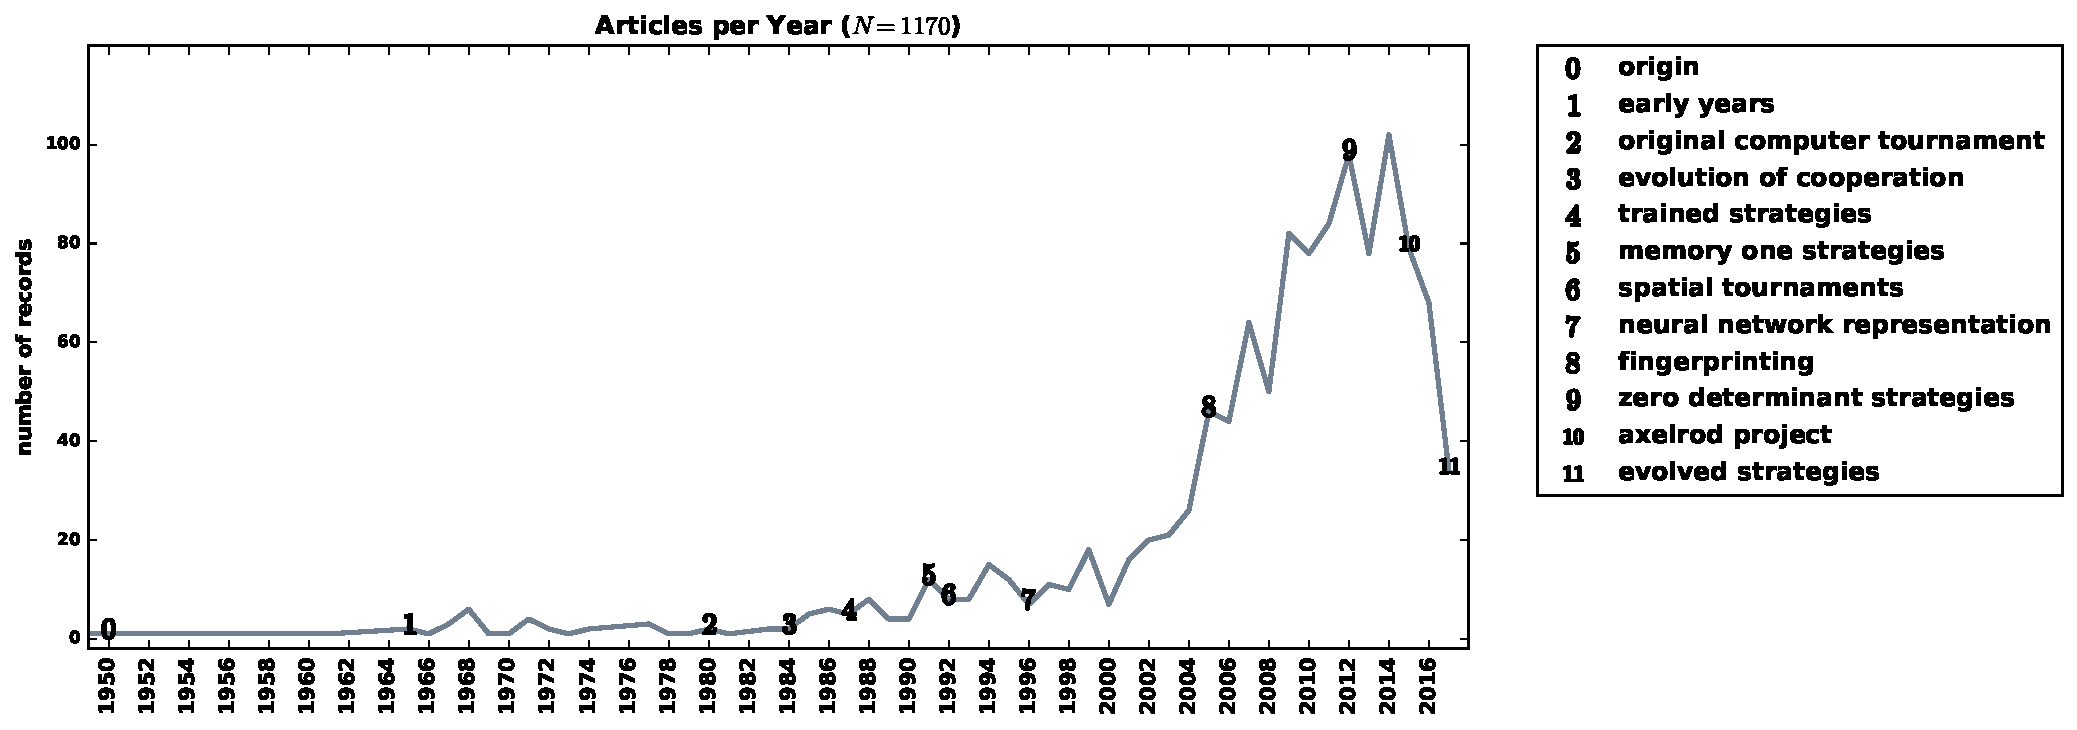
\includegraphics[width=\textwidth]{assets/images/timeline.pdf}
    \caption{\label{fig:timeline} A timeline of the prisoner's dilemma research.}
\end{figure}

\section{Timeline}\label{section:timeline}

\subsection{Origin and Primal research (1961-1972)}

The origin of the prisoner's dilemma goes back to the 1950s in early experiments
conducted in RAND~\cite{Flood1958} to test the applicability of games
described in~\cite{VonNeumann1944}. Although the name behind the game was given
later the same year.
According to~\cite{Tucker1983}, A. W. Tucker (the PhD supervisor of J. Nash),
in an attempt to delivery the game with a story during a talk used prisoners as
players and the game has been known as the prisoner's dilemma ever since.

The study of the prisoner's dilemma has attracted people from various fields
across the years. An early figure within the field is Prof A. Rapoport,
a mathematical psychologist, whose work focused on peacekeeping.
In his early work~\cite{rapoport1965} Rapoport conducted experiments using humans
to simulate a play of the prisoner's dilemma. Experimental groups were not been
used only by Rapoport but it was a common mean of studying the game
\cite{Evans1966, Gallo1968, Lutzker1961, Mack1971, Sensenig1972} and are still
being used today. %TODO reference a good article with human studies.

Those experiments explored the conditions under which altruist behaviour emerges
in human societies. Conditions such as, the gender~\cite{Evans1966,
Lutzker1961, Mack1971} of individuals, the representation of the game
\cite{Evans1966}, the distance between players~\cite{Sensenig1972}, the initial effects
\cite{Tedeschi1968} and whether the experimenter was biased~\cite{Gallo1968}.

Even though, several of these experiments were held and continuous research on
the topic was undergoing game theorists were still in disagreement about
the best way to play the game~\cite{rapoport1965}. Inspired by the work of
Rapoport and intrigued by the very same question the political scientist R.
Axelrod took upon himself to identify the dominant strategy of the prisoners dilemma.

The main difference of Axelrod's approach was that machines were going to be used
instead of humans. The issues with using humans, according to Axelrod
\cite{Axelrod2012}, was the fact that humans can act very randomly even though
the aim of the game is clear to them. Thus, Axelrod was the first researcher,
to the author's knowledge, to perform a computer tournament of the iterated
prisoner's dilemma. The tournaments and their results are discussed in
the next sections.

\subsection{Axelrod's Tournaments (1981-1984)}\label{subsection:axelrods_tournament}

This section serves as a follow up from the earlier years of the topic and as an
introduction to the modern ways of studying the prisoner's dilemma. It is
dedicated to the computer tournaments of R. Axelrod from 1981 to 1984.

The first computer tournament was performed in 1980~\cite{Axelrod1980a}.
Several scientists were invited to submit their strategies, written in the
programming languages Fortran or Basic. There was a total of 13 submissions
made by the following researchers,

\begin{multicols}{2}
    \begin{enumerate}
        \item T Nicolaus Tideman and Paula Chieruzz;
        \item Rudy Nydegger;
        \item Bernard Grofman;
        \item Martin Shubik;
        \item Stein and Anatol Rapoport;
        \item James W Friedman;
        \item Morton Davis;
        \item Jim Graaskamp;
        \item Leslie Downing;
        \item Scott Feld;
        \item Johann Joss;
        \item Gordon Tullock;
        \item Name not given.
    \end{enumerate}
\end{multicols}

Each competed in a 200 turn match against all 13 opponents, itself and a player
that played randomly. This type of tournament is referred to as a round robin and
corresponds to a complete graph from a topological point of view. The tournament
was repeated \(5\) times to reduce variation in the results. Each participant knew
the exact length of the matches and had access to the full history of each match.
Furthermore, Axelrod performed an preliminary tournament and the results were known
to the participants. The payoff values used for equation(\ref{eq:the_pd_payoffs}) where
\(R=3, P=1, T=5\) and \(S=0\). These values are commonly used in the literature
and unless specified will be the values used in the rest of the work described here.

The winner of the tournament was determined by the total average score and not by
the number of matches won. The strategy that was announced the winner was
submitted by Rapoport and was called \textbf{Tit For Tat}. Tit for Tat, is a
strategy that always cooperates on the first round and then mimics the opponent's
previous move.

Examples of Tit for Tat interacting for 8 turns with deterministic opponents are
given by Tables~\ref{table:tft_vs_c}, \ref{table:tft_vs_d} and \ref{table:tft_vs_a}.
The opponents are, \textbf{Cooperator} a strategy that always cooperates,
\textbf{Defector} an opponent that always defects and \textbf{Altenator} a
player who alternates between cooperating and defecting.

\begin{table}[!hbtp]
    \begin{center}
    \begin{tabular}{lcc}
        \toprule
        Turns & Tit for Tat & Cooperator\\
        \toprule
        1 & C & C \\
        2 & C & C \\
        3 & C & C \\
        4 & C & C \\
        5 & C & C \\
        6 & C & C \\
        7 & C & C \\
        8 & C & C \\
        \bottomrule
    \end{tabular}
    \caption{Tit for Tat example match of 8 turns against Cooperator}\label{table:tft_vs_c}
    \end{center}
\end{table}

\begin{table}[!hbtp]
    \begin{center}
    \begin{tabular}{lcc}
        \toprule
        Turns & Tit for Tat & Defector\\
        \toprule
        1 & C & D\\
        2 & D & D\\
        3 & D & D\\ 
        4 & D & D \\
        5 & D & D\\
        6 & D & D\\ 
        7 & D & D \\
        8 & D & D \\
        \bottomrule
    \end{tabular}
    \caption{Tit for Tat example match of 8 turns against Defector}\label{table:tft_vs_d}
\end{center}
\end{table}

\begin{table}[!hbtp]
    \begin{center}
    \begin{tabular}{lcc}
        \toprule
        Turns & Tit for Tat & Altenator\\
        \toprule
        1 & C & C \\ 
        2 & C & D \\ 
        3 & D & C \\ 
        4 & C & D \\
        5 & D & C \\ 
        6 & C & D \\ 
        7 & D & C \\ 
        8 & C & D \\
        \bottomrule
    \end{tabular}
    \caption{Tit for Tat example match of 8 turns against Altenator}\label{table:tft_vs_a}
\end{center}
\end{table}

The results of the first tournament were filled with surprises. Tit for Tat the
simplest strategy of all had won and had managed to defeat even entrants that
tried to improve on Tit for Tat after the preliminary tournament results.
Axelrod justified the success of the strategy saying that the strategy was
`nice' and `forgiving'.

The top eight ranked strategies were strategies that did no defect on the first
round, thus they were described as `nice' strategies. Compared to the rest of the
"nice" strategies, Tit for Tat had also another property. That property was
`forgiveness'. Tit for Tat punished it's opponent for a defection but just once
and then it would try to cooperate again. These two properties were described to
be the secret of success in a prisoner's dilemma tournament.

In order to further test the robustness of the results Axelrod performed a second
tournament~\cite{Axelrod1980b} later in 1980. This time a total of 63 participants
submitted strategies, their names were the following,

\begin{multicols}{3}
    \begin{enumerate}
        \item Gail Grisell;
        \item Harold Rabbie;
        \item James W Friedman;
        \item Abraham Getzler;
        \item Roger Hotz;
        \item George Lefevre;
        \item Nelson Weiderman;
        \item Tom Almy;
        \item Robert Adams;
        \item Herb Weiner;
        \item Otto Borufsen;
        \item R D Anderson;
        \item William Adams;
        \item Michael F McGurrin;
        \item Graham J Eatherley;
        \item Richard Hufford;
        \item George Hufford;
        \item Rob Cave;
        \item Rik Smoody;
        \item John Willaim Colbert;
        \item David A Smith;
        \item Henry Nussbacher;
        \item William H Robertson;
        \item Steve Newman;
        \item Stanley F Quayle;
        \item Rudy Nydegger;
        \item Glen Rowsam;
        \item Leslie Downing;
        \item Jim Graaskamp and Ken Katzen;
        \item Danny C Champion;
        \item Howard R Hollander;
        \item George Duisman;
        \item Brian Yamachi;
        \item Mark F Batell;
        \item Ray Mikkelson;
        \item Craig Feathers;
        \item Fransois Leyvraz;
        \item Johann Joss;
        \item Robert Pebly;
        \item James E Hall;
        \item Edward C White Jr;
        \item George Zimmerman;
        \item Edward Friedland;
        \item X	Edward Friedland;
        \item Paul D Harrington;
        \item David Gladstein;
        \item Scott Feld;
        \item Fred Mauk;
        \item Dennis Ambuehl and Kevin Hickey;
        \item Robyn M Dawes and Mark Batell;
        \item Martyn Jones;
        \item Robert A Leyland;
        \item Paul E Black;
        \item T Nicolaus Tideman and Paula Chieruzz;
        \item Robert B Falk and James M Langsted;
        \item Bernard Grofman;
        \item E E H Schurmann;
        \item Scott Appold;
        \item Gene Snodgrass;
        \item John Maynard Smith;
        \item Jonathan Pinkley;
        \item Anatol Rapoport.
    \end{enumerate}
\end{multicols}

All the participants knew the results of the previous tournament. The rules
were similar to those of the first tournament with only one exception;
the number of turns was not specified instead a fixed probability (refereed to as
`shadow of the future'~\cite{Axelrod1988}) of the game ending on the next move
was used. The fixed probability was chosen to be 0.0036 so that the expected
median length of a match would be 200 turns. The topology was of a round robin
and each pair of players was matched 5 times. Each of the five matches had a
length of 63, 77, 151, 308 and 401.

The first tournament had reported that it paid for a strategy to be nice and forgiving.
These ideas were carried onto the second tournament from various applicants.
A total of 39 strategies were now nice and nearly all of them somewhat forgiving.
There were also two lessons taken from the report of the first tournament:

\begin{enumerate}
    \item Be nice and forgiving.
    \item If others are going to be nice and forgiving take advantage of them.
\end{enumerate}

The strategies that based their behaviour on lesson one suffered due to lesson
two. The strategies following lesson two suffered while trying to exploit their
opponents. The most successful entries tended to be variants of Tit for Tat,
such as \textbf{Tit for Two Tats} submitted by John Maynard Smith. Tit for Two
Tats defects only when the opponent has defected twice in a row. However
none of the variants managed to outperform the pure version. All that said
the winner of the second tournament was once again Tit for Tat. The conclusions
of~\cite{Axelrod1980a} were that the strong performance of the strategy was due to:

\begin{itemize}
    \item The strategy would start of by cooperating.
    \item It would forgive it's opponent after a defection.
    \item It would always be provoked by a defection no matter the history.
    \item As soon as the opponents identified that they were playing Tit for Tat,
    they would choose to cooperate for the rest of the game.
\end{itemize}
%The strategies of the second tournament where bias due the first tournament. Discuss with V.
These characteristics allowed Tit for Tat to achieve the highest average score
over the 63 rules in the tournament. The repeated success of the strategy soon raised
a question: Is Tit for Tat the best strategy when playing the iterated prisoner's dilemma? 

So far it has been discussed how the performance of the strategy has been tested
through tournaments against other strategies. But is the overall success of a
strategy based only on it's performance in a round robin tournament or should
it be checked through other ways as well? R. Axelrod asking the very same question
performed an `ecological' tournament in 1981~\cite{Axelrod1984}.

Axelrod argued that some strategies are so unsuccessful that there are very likely
to be dropped in the future, while other more successful strategies would continue
in later interactions. Influenced by evolutionary biology Axelrod introduced a way
of capturing this behaviour, which included running a series of tournaments where
more successful strategies would occupy a larger part of the environment and the
less successful strategies would become less often. This is known as an ecological
tournament.

The simulation of the process, as described in~\cite{Axelrod1984}, is straightforward.
Consider matrix~\ref{eq:interaction_payoffs} which provides the expected payoff
when two individuals of different types interact. Starting with proportions of
each type in a given generation the proportions of these strategies in the next
generation is the only measure we need to calculated. This is achieved by
calculating the weighted average of the scores of a given strategy with all
other players. The weights are the numbers of the other strategies which
exist in the current generation. The numbers of a given strategy in the next
generation is then taken to be proportional to the product of its numbers in the
current generation and its score in the current generation.

\begin{equation} \label{eq:interaction_payoffs}
    \begin{pmatrix}
    (R=3, R=3) & (S=0, T=5) \\ (T=5, S=0) & (P=1, P=1)
    \end{pmatrix}
\end{equation}

Note that the ecological tournament does not offer any evolutionary perspective.
There is no possibility of a new strategy to be introduced, there is no mutation
probability to drive the evolution. The ecological tournament is a framework that provides
the distributions of given types over time when interacting with the population.

The set of strategies from Axelrod's second tournament was used to perform the
ecological tournament. Several interesting insights were reported,

\begin{itemize}
    \item The lowest ranking 11 strategies had fallen to half their initial size
    by the 5 generation;
    \item The middle-ranking entries managed to hold their initial size;
    \item By the \(500^{th}\) generation the only strategies that were larger than their
    initial size have been the top 11 ranked strategies;
    \item These formed 96\% of the population at that time;
    \item The rule which ranked fifth in the tournament, submitted by William Adams,
    grew to three times its original size in the population and then began to sink
    after generation 100;
    \item The rule which ranked eighth, submitted by Paul D. Harrington, and was
    the only non nice rule in the top 15, grew to four times its original size but
    began to shrink after generation 150 to reach only a third of its original
    size by the \(1000^{th}\) generation.
\end{itemize}

Overall the strategies that did rank at the top of the second tournament have
also ranked top in the ecological tournament. On the same note, the strategy that
was ranked at the top was again Tit for Tat. By the 1000th generation it was 14.5\%
of the whole population, followed by the third place rule at 13.9\% and then the
second place rule at 13.1\%. Tit for Tat was growing at .05\% per generation which
was a faster rate than any other strategy. All these are captured by
Figure~\ref{fig:ecological.tournament}.
% This is a lie. We said that the table would make more sense here.

\begin{figure}[!hbtp]
    \centering
    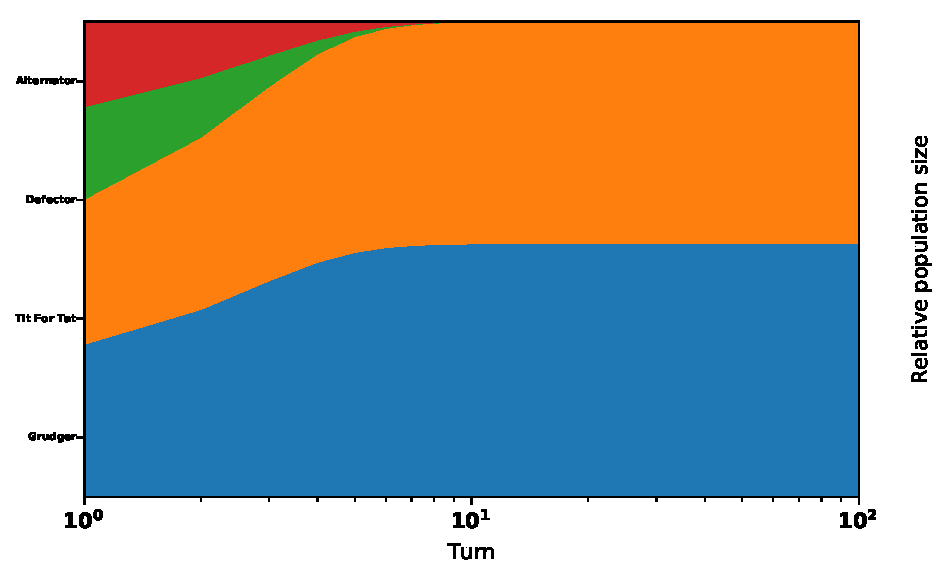
\includegraphics[width=.6\textwidth]{./assets/images/ecological.pdf}
    \caption{System evolving over time based on natural selection using
    \cite{axelrodproject}, strategies set from Axelord's second tournament.}
    \label{fig:ecological.tournament}
\end{figure}

A much more general approach was discussed in~\cite{axelrod1981}; the evolutionary
approach. Imagine a population made up of individuals where everyone follows the
same strategy, \(B\) and a single individual adopts a mutant strategy \(A\).
Strategy \(A\) is said to invade strategy \(B\) if,

\begin{equation}
V(A \mid B) > V(B \mid B)
\end{equation}
where \(V(B \mid B)\) is the expected payoff received by \(B\) against itself.

Since the strategy \(B\) is an population that interacts only with itself,
the concept of invasion is equivalent to a single mutant being able to outperform
the average population. This leads to the concept of the evolutionary approach.
Thus for a strategy to be \textbf{evolutionary stable} it must be able to
resists any invasion. There are several applications in biology for the interpretation
of this approach, for example the survival of the fitness in wildlife.

The ability of strategies to be favoured under natural selection and their
ability to withstand invasion from other strategies soon became a measure
of performance; refereed to as the stability of a strategy.

Due the large number of possible strategies in the prisoner's dilemma identifying
all the stable strategies was a difficulty task at the time. Axelrod focused
the work of~\cite{axelrod1981} in three questions,

\begin{enumerate}
    \item Under what conditions was Tit for Tat evolutionary stable?
    \item What were the necessary and sufficient conditions for any strategy to be
    evolutionary stable?
    \item Finally, in an environment where all followed a strategy of unconditional
    defection, can cooperation emerge?
\end{enumerate}

A series of theorems were presented which showed, that Tit for Tat is evolutionary
stable if and only if it is invadable neither by Defector nor Alternator. This
is true only if the game is likely to last long enough for the retaliation
to counteract the temptation to defect, according to Axelrod. Secondly,
Defectors can withstand invasion by any strategy, as long as the players using
other strategies come one at a time. But if they come in clusters (even in rather small
clusters), the strategy could be invaded. As for the characteristics of stable
strategies, Axelrod provided a series of theorems.

Overall, all of Axelrod's tournaments offered many insights and new concepts to the field.
These were not only limited on Tit for Tat. For example several strategies of
these tournaments are still being used in literature to date, such as Tit for
Two Tats and \textbf{Grudger}.

Grudger was originally submitted by James W. Friedman. Grudger is a strategy that
will cooperate as long as the opponent does not defect. The name Grudger was give
to the strategy in~\cite{Li2014}. Though the strategy goes by many names in the
literature such as, Spite~\cite{Beaufils1997}, Grim Trigger~\cite{Banks1990} and
Grim~\cite{Van2015}.

Though not all strategies of Axelrod's tournament are retrievable. The author
had given a explanation of all 13 strategies of the first tournament.
The size of the second tournament did not allow him this time to go into details
for every single participant. The author mainly focused on the high ranked participants.
However, the source code of the 63 strategies can be found on Axelrod's personal
website~\cite{fortan_code}. Figure~\ref{fig:tit_for_tat_fortran} serves as an
example of the source code for the winning strategy Tit for Tat.

\begin{figure}[!hbtp]
    \centering
    \begin{minted}
        [
        autogobble=true,
        framesep=2mm,
        fontsize=\normalsize,
        ]
        {fortran}
    FUNCTION K92R(J,M,K,L,R, JA)
C BY ANATOL RAPOPORT
C TYPED BY AX 3/27/79 (SAME AS ROUND ONE TIT FOR TAT)
c replaced by actual code, Ax 7/27/93
c  T=0
c   K92R=ITFTR(J,M,K,L,T,R)
      k92r=0
      k92r = j
c test 7/30
c   write(6,77) j, k92r
c77   format(' test k92r. j,k92r: ', 2i3)
      RETURN
      END
    \end{minted}
    \caption{\label{fig:tit_for_tat_fortran} Source code for Tit for Tat in Fortran.
    Provided by~\cite{fortan_code}.}
\end{figure}

Note though that the code of the second tournament only includes the strategies.
The code for running a round robin tournament or an ecological tournament
is not given. Moreover, the source code of the first 13 strategies is not
available, as stated in Axelrod's personal website~\cite{fortan_code}.

\subsection{Response to the computer tournaments (1984-1993)}
\label{section:responses_to_computer_tournament}

The pioneering work of computer tournaments and the results of the reciprocal behaviour
in the prisoner's dilemma spread the knowledge of the game worldwide and across
disciplines. Several researchers responded immediately to Axelrod's tournaments
and the study of cooperation became of critical interest once again.
This section focuses on the research that was carried out after the initial
computer tournaments. More specifically the research the falls in the following
categories, over the time period between 1984 and 1993, are considered in this section:

\begin{itemize}
    \item Applications of the iterated prisoner's dilemma, the famous strategy
    Tit for Tat and the reciprocal behaviour.
    \item Computer tournaments under stochastic uncertainty and the introduction
    of new strategies.
\end{itemize}

One of the scientific disciplines that immediately employed Axelrod's work has
been the ecological field. More specifically, the works of~\cite{Craig1984,
Dugatkin1988, Godfray1992, Milinski1987, Wilkinson1984}.
In~\cite{Dugatkin1988, Milinski1987} the behaviour of fish when confronting a
potential predator was studied. Conflicts can arise within pairs of fish in these
circumstances. In both works experiments were held using a system of mirrors
where sticklebacks and guppies respectively, would be accompanied by a cooperating
companion or a defecting one. In both cases the hypothesis that the fish would
behave according to Tit for Tat and that cooperation would evolve was supported.
The works of~\cite{Godfray1992, Wilkinson1984} looked at food sharing between
vampire bats and explained behaviour based on known strategies.

Another quick response to the tournaments was that of~\cite{Molander1985}.
It was argued that Axelrod's work assumed that each player had a perfect
information of the opponent's actions. In real life situations this is not always
the case. Interactions often suffer from measures of uncertainty and this was not
captured in the original tournaments. Molander studied the performance of Tit for
Tat in an uncertain environment by introducing noise. A probability that a player's
move will be flipped. It was proven that when two strategies playing Tit for Tat
met in a noisy match the average payoff of each strategy would be the same as
that of a Random player (with a probability \(0.5\) of cooperating).

In 1988 publications from other disciplines were using the iterated prisoner's
dilemma and Axelrod's work for teaching and social studies.
In~\cite{Levitt1988} a version of the prisoner's dilemma which set the
problem in an ordinary business context was used as a pedagogic instrument within
graduate business students. The work of~\cite{Rabow1988} considered non zero sum
games, specifically the prisoner's dilemma, and illustrated the impact they
have on societal problems such as war.

In 1989 reactive strategies are introduced in~\cite{nowak1989}. Reactive strategies
are a set of players that take into account only the last move of the opponent. 
Thus, they can be represented by the probability of cooperating after an opponent's
\textbf{C} or \textbf{D}. The same author a year later in 1990 gave a formal
definition of a memory one~\cite{Nowak1990}. Memory one strategies consider the
entire history of the previous turn to make a decision. Thus reactive strategies are
a subset of memory one.

If only a single turn of the game is taken into account and depending on the
simultaneous moves of two players there are only four possible states that
players could possibly be in. These are \(CC, CD, DC\) and \(DD\). A memory one
strategy is denoted by the probabilities of cooperating after each of these states,
\( p = (p_1, p_2, p_3, p_4) \in\mathbb{R}_{[0,1]}^{4} \).
A match between two memory one players \(p\) and \(q\) can be modelled as a
stochastic process, where the players move from state to state. More specifically,
it can be modelled by the use of a Markov chain, which is described by a matrix 
\(M\).

\begin{equation}\label{eq:markov_matrix}
    M =
\begin{bmatrix}
    p_{1} q_{1} & p_{1} (- q_{1} + 1) & q_{1} (- p_{1} + 1) & (- p_{1} + 1) (- q_{1} + 1)
    \\
    p_{2} q_{3} & p_{2} (- q_{3} + 1) & q_{3} (- p_{2} + 1) & (- p_{2} + 1) (- q_{3} + 1)
    \\
    p_{3} q_{2} & p_{3} (- q_{2} + 1) & q_{2} (- p_{3} + 1) & (- p_{3} + 1) (- q_{2} + 1)
    \\
    p_{4} q_{4} & p_{4} (- q_{4} + 1) & q_{4} (- p_{4} + 1) & (- p_{4} + 1) (- q_{4} + 1)
    \\
\end{bmatrix}
\end{equation}

The players are assumed to move from each state until the system reaches a state
steady.  The utility of a player can be given by multiplying the steady states of
\(M\) by the payoffs of equation(\ref{eq:the_pd_payoffs}). Thus~\cite{Nowak1990}
offered a mathematical framework to calculate the utility of two players without
simulating the game. Memory one strategies are considered an important family of
strategies and the formulation given in 1990 is still being used to date.

A player called \textbf{Handshake} was presented by~\cite{Robson1989} in 1989.
Handshake is a strategy that starts with cooperation, defection. If the opponent
plays in a similar way then it will cooperate forever, otherwise it will defect
forever. Handshake has a property that will be revisited in this literature
review which is it's recognition property.

From 1991 to 1992, further research explored the performance of Tit for Tat in uncertain
environments. These works include~\cite{Godfray1992, Bendor1991, Nowak1992}.
In~\cite{Bendor1991} a similar tournament to that of Axelrod's was performed,
but this time it was a noise tournament. Bendor had invited researchers from several
departments across his university and from a university seminar. Each match
would last a random number of turns, with a probability of 0.0067 of ending in
the next turn. The probability of noise was a random variable, distributed normally
with a mean of zero and a standard deviation of eight. The results of his
tournament demonstrated that Tit for Tat performed rather poorly and the highest
ranked strategies were generous ones. The top ranked strategy was \textbf{Nice and Forgiving}.

The work of~\cite{Nowak1992} aimed to also investigate stochastic effects.
This is was done using an evolutionary setting of a heterogeneous population
with noise. The author investigate which strategies would manage to take over
the population and would be evolutionary stable. The strategies were explored
over the space of reactive strategies. The results demonstrated that 
though a small fraction of Tit for Tat players have been essential for the emergence
of cooperation, more generous strategies took over the population. More specifically
the re active strategy known as \textbf{Generous Tit for Tat} which is presented as
\((0, \frac{2}{3})\).

The author of~\cite{Nowak1992, nowak1989, Nowak1990} also introduced another
important strategy of the literature. It was presented in~\cite{Nowak1993} and
is it known as \textbf{Pavlov}. Pavlov is a strategy with the tolerance of Generous Tit for Tat
but also the capability of resisting and invading an all-out cooperators population.
The strategy is based on the fundamental behavioural mechanism win-stay,
lose-shift. It starts off with a cooperation and then repeats it's previous move
only if it was awarder with a payoff of \(R\) or \(T\). Otherwise it shifts
it's last move.
 
\subsection{Evolutionary Dynamics (1987-1999)}
% This needs work I know
Determining the evolutionary stability of strategies for the iterated prisoner's
dilemma as we discussed is not an easy task. Methods can be use to deal with
the difficulty. In~\cite{Boyd1987} the author restricted the possible strategies
that could be adopted to a relatively narrow set and resulted that no pure strategy
is evolutionary stable, including Tit for Tat. Arguing with the results presented
in~\cite{axelrod1981}. The list of strategies used included strategies such as
Defector and \textbf{Suspicious Tit for Tat}, a strategy that plays
Tit for Tat but starts by defecting.

The results were questioned by~\cite{May1987}, stating that much was still no fully
explored and more research had to be put into the results. Farrel and Ware in
1989~\cite{Farrell1989} extended the result to include finite mixture of pure
and mixtures of Tit For \(n\) Tats as well. On the same year the work of~\cite{Boyd1989}
looking again at a narrow set of strategies extended their results to
noisy environments.

Evolutionary dynamics have been highly useful in the research of the prisoner's
dilemma. In~\cite{Axelrod1987}, an evolutionary process, called the genetic
algorithm, was used to discover effective strategies. The author introduced
lookup tables as a mean of representing a strategy in a gene format. A lookup
table is a set of deterministic responses based on the opponents \(m\) last
moves; \cite{Axelrod1987} considered \(m=3\).

An extension to the natural selection was introduced in the 1992~\cite{Nowak1992b},
recommending a different type of topology. A population of two deterministic
strategies, Defector and Cooperator, were placed on a a two dimensional square array
where the individuals could interact only with the immediate neighbours.
The number of immediate neighbours could be either, fourth, six or eight. As
shown in Figure~\ref{fig:topologies}. The authors claimed that the essential
results remain true of all topologies; the results also hold whether self interactions
are taken into account.

Thus each cell of the lattice is occupied by a Cooperator or a Defector. At
each generation step each cell owner interacts with its immediate neighbours.
The score of each player is calculated as the sum of all the scores the player
achieved at each generation. At the start of the next generation, each lattice
cell is occupied by the player with the highest score among the previous owner
and the immediate neighbours. This topology is refereed to as spatial topology.

Nowak studied the population dynamics as a function of the temptation payoff.
It was shown that for different values of the temptation payoff, cooperators
and defectors could persist together.

\begin{figure}[!hbtp]
\centering
    \begin{subfigure}{.25\textwidth}
        \hspace{.8cm}
        \includestandalone[width=0.6\textwidth]{assets/tex/neighb_four}
    \end{subfigure}
    \begin{subfigure}{.25\textwidth}\centering
        \includestandalone[width=0.6\textwidth]{assets/tex/neighb_eight}
     \end{subfigure}
     \begin{subfigure}{.25\textwidth}\centering
        \includestandalone[width=0.6\textwidth]{assets/tex/neighb_six}
     \end{subfigure}
    \begin{subfigure}{.25\textwidth}
        \includestandalone[width=\textwidth]{assets/tex/square_lattice}
    \end{subfigure}
    \begin{subfigure}{.25\textwidth}\centering
        \includestandalone[width=\textwidth]{assets/tex/square_lattice_eight}
     \end{subfigure}
     \begin{subfigure}{.25\textwidth}\centering
        \includestandalone[width=\textwidth]{assets/tex/hexagonal_lattice}
     \end{subfigure}
     \caption{Spatial neighbourhoods}\label{fig:topologies}
    \end{figure}

This work dealt with dealt with symmetric spatial lattices in two dimensions,
deterministic winning and discrete time. The authors in later work~\cite{nowak1994},
that the results remain valid in more realistic situations. Such as situations
where the spatial distributions of cells are random in two or three dimensions,
and where winning is partly probabilistic.

\subsection{Modern approaches (1995-2015)}\label{section:modern_approaches}

In this section we will cover several research projects published between 1995
and 2015. The research reviewed here focuses on computer tournaments and serves
as an introduction to various strategies that have made an impact in the literature.

Initially in 1995 a combination of tournament studies, ecological simulations
and theoretical analysis was used in~\cite{Wu1995} to demonstrate approaches on
coping with noise. The first approach was \textit{generosity}. A more generous version
of Tit for Tat, the strategy called the Generous Tit for Tat, was proven to be
highly effective against players that were not adapted to noise. The second
approach introduced was \textit{contrition}. The authors stated that when
interacting with strategies that have been adapted to noise a contrite version 
of Tit for Tat is even more effective at quickly restoring mutual cooperation 
without the risk of exploitation. The strategy introduced as the contrite variant
was called \textbf{Contrite Tit for Tat}. A strategy which three states:
\textit{contrite, content, provoked}. It begins by cooperating and stays there unless
there is a unilateral defection. If it was the victim of a defection while content
the strategy becomes provoked and defects until the opponent cooperates, and 
causes it to become content. If it was the defector while content, it
becomes contrite and cooperates. When contrite it becomes content only after
there has been a mutual cooperation. The final approach has been using strategy
Pavlov. Moreover, in the analysis an variant of Pavlov was also included
called Generous Pavlov, a variant that cooperates 10\% of the times when it 
would either wise had defected. Though all approaches were effecting in coping
with noise in a standard tournament, the authors argued that Pavlov was not 
suited for ecological tournaments.

An interesting approach of to capture promising strategies for the game
was written in 1996 by~\cite{Miller1996}. Strategies represented by finite automata
were learning to update their choices through an explicit evolutionary process
modelled by a genetic algorithm.

Strategies based on finite state machines are described by the number of states.
The strategy selects the next action in each round based on the current state
and the opponent's last move, transitioning to a new state each time.
Figure~\ref{fig:tit_for_tat_fsm}, illustrates the finite state representation
of Tit For Tat.

\begin{figure}[!hbtp]
    \centering
    \includestandalone[width=.3\textwidth]{./assets/tex/tit_for_tat_fsm}
    \caption{Finite state machine representation of Tit for Tat.}
    \label{fig:tit_for_tat_fsm}
\end{figure}

In 1997, \textbf{Gradual} a well performed strategy and a commonly known in the
literature was proposed by~\cite{Beaufils1997}. Gradual starts off by cooperating,
then after the first defection of the other player, it defects one time and cooperates
twice. After the second defection of the opponent, it defects two times and cooperates
twice. After the \(n^{th}\) defection it reacts with \(n\) consecutive defections 
and then two cooperations. Gradual had managed to outperform strategies such
as Tit for Tat and Pavlov.

Though several of this tournament discussed so far were generated using computer
code not all of the source code was made available by the authors. Several
open projects were created and published through the year. The first one
discussed in this work, excluding the code for Axelrod's strategies, is 
PRISON~\cite{prison}. PRISON is written in the programming language Java and
preliminary version was launched on 1998. It was used by it's authors in several
publications. The project includes a good number of strategies from the
literature but unfortunately the last update of the project dates back in 2004.

Another measure of uncertainty discussed in 1998~\cite{Hoffmann1998} is that of
mis perception. Mis perception is the probability that the opponent's current
move is flipped before being recorded to the history. Results of~\cite{Hoffmann1998}
indicated that noise effected the emergence of cooperative behaviour in the
populations. In 1999, \cite{Turner1999} uses evolutionary game theory to study
the spread of virus.

Following the success of Gradual the authors of~\cite{tzafestas-2000a}
conducted a tournament of 13 strategies just to outperform it. Their strategy
was the \textbf{Adaptive Tit for Tat} and the algorithm used by it is given by
\ref{alg:adaptive_tft}.

\begin{algorithm}
\begin{algorithmic}[1]
    \IF{opponent played \textbf{C} in the last cycle}
     \STATE world = world + \(r(1-\text{world})\), \(r\) is the adaptation rate
    \ELSE
     \STATE work = world + \(r(0 - \text{world})\)
     \ENDIF
    \IF{world \(\geq\) 0.5}
        \STATE play \textbf{C}
    \ELSE
    \STATE play \textbf{D}
    \ENDIF
\end{algorithmic}
\caption{Adaptive Tit for Tat.}
\label{alg:adaptive_tft}
\end{algorithm}

Adaptive Tit for Tat ranked first in it's tournament surpassing Gradual. However,
the results were drawn from a tournament of 13 strategies.

% Less generous variants also made an appearance~\cite{Hilde2013}.
% \textbf{Anti Tit for Tat}, is a strategy that plays the opposite of the opponents
% previous move. Another limitation of the strategy was discussed in~\cite{Wolfgang2006}.
% Tit for Tat was proven to hit a loop between cooperation and defection.
% \textbf{Omega Tit For Tat} was introduced and was a strategy capable of avoiding
% such problem~\cite{Wolfgang2006}.

In~\cite{Ashlock2006b} the author presented two new strategies that have
been trained using a finite state machine representation. They are called,
\textbf{Fortress3} and \textbf{Fortress4}. Figure~\ref{fig:fortress3_and_4}
illustrates their diagrammatic representation where the transition arrows are
labelled \textit{O/P} where \textit{O} is the opponent's last action and \textit{P}
is the player's response.

\begin{figure}[!hbtp]
\centering
    \begin{subfigure}{.4\textwidth}
        \includestandalone[width=\textwidth]{assets/tex/fortress_3}
    \end{subfigure}
    \begin{subfigure}{.4\textwidth}\centering
        \includestandalone[width=\textwidth]{assets/tex/fortress_4}
     \end{subfigure}
     \caption{Representations of Fortress 3 and Fortress 4. Note that the
     strategy's first move, enters state 1, is defection for both strategies.}
     \label{fig:fortress3_and_4}
\end{figure}

Optimisation methods return a spectrum of strategies. In order to distinguish
the strategies and assuring that they are indeed different~\cite{Ashlock2005}
introduced a method called fingerprinting.

The method of fingerprinting is a technique for generating a functional signature for a
strategy~\cite{Ashlock2008}. This is achieved by computing the score of a strategy
against a spectrum of opponents. The basic method is to play the strategy
against a probe strategy with varying noise parameters. In~\cite{Ashlock2005}
Tit for Tat is used as the probe strategy. Fingerprint functions
can then be compared to allow for easier identification of similar strategies.
In Figure~\ref{fig:fingerprinting} an example of Pavlov's fingerprint is given.
Fingerprinting has been studied in depth in~\cite{Ashlock2008, Ashlock2009,
Ashlock2010, Ashlock2006a}.

\begin{figure}[!hbtp]
    \centering
    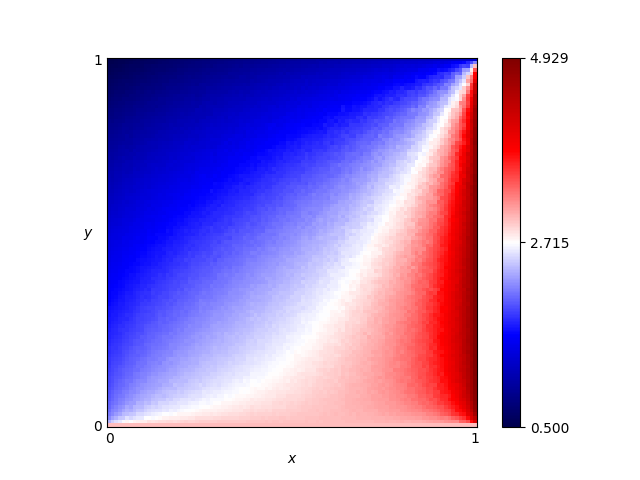
\includegraphics[height=.3\textheight]{./assets/images/Win-Stay_Lose-Shift.png}
    \caption{Pavlov fingerprinting with Tit for Tat used as the probe strategy.
    Figure was generated using~\cite{axelrodproject}.}
    \label{fig:fingerprinting}
\end{figure}

The adaptive behaviour that was tried to be capture by~\cite{tzafestas-2000a}
was not constrained only on Tit for Tat. In~\cite{Li2011} \textbf{APavlov},
which stands for adaptive Pavlov, made an appearance.  The strategy attempts to
classify the opponent as one of the following strategies, All Cooperator,
All Defector, Pavlov, Random or \textbf{PavlovD}. PavlovD, is just Pavlov
but it starts the game with a \textbf{D}. Once Adaptive Pavlov has classified
the opponent plays to maximize it's payoff.

In 2011 the authors of~\cite{Li2011} performed their own tournament where
several interesting strategies made an appearance.

\begin{itemize}
    \item \textbf{Periodic player CCD}, plays \textbf{C}, \textbf{C}, \textbf{D}
    periodically. Note that variations of a period player also make appearance
    in the article but will not be listed here.
    \item \textbf{Prober}, starts with the pattern \textbf{D}, \textbf{C}, \textbf{C}
     and then defects if the opponent has cooperated in the second and third move;
     otherwise, it play as Tit for Tat.
    \item \textbf{Reverse Pavlov}, a strategy that does the reverse of Pavlov.
\end{itemize}

\subsection{Zero determinant (2012 - 2015)}

In 2012 Press and Dyson~\cite{Press2012} studied the iterated prisoner's dilemma and presented
a new set of strategies called \textbf{zero determinant (ZD)}. The ZD strategies
are memory one strategies that manage to force a linear relationship between their
score and that of the opponent.

In Section~\ref{section:responses_to_computer_tournament} it was described how
the payoffs of two players could be retrieved by formulating their interactions
using a Markov chain. Let us denote the payoffs of players \(p\) and \(q\) as:

\begin{align*}
    s_p = v S_p \\
    s_q = v S_q
\end{align*}

where \(v\) is a vector of the steady states of matrix \(M\) and \(S_p\), \(S_q\)
are the equivalent payoff values of the players for each state \(CC, CD, DC, DD\).
Using linear algebra, Press and Dyson showed that the dot product of the stationary
distribution of \(v\) with any vector \(f\) can be expressed as a \(4\times 4\)
determinant. In which one column is \(f\), one column is entirely under the control
of player \(p\) and another column is entirely under the control of player \(q\).

This meant that either \(p\) or \(q\) could independently force the dot product
of \(v\) with some other chosen vector \(f\) to be zero by choosing their
strategy so as to make the column they control be proportional to \(f\).
In particular, by \( f = \alpha S_p + \beta S_q + \gamma\), any player can force
a given linear relation to hold between the long-run scores of both players.

Press and Dyson's results suggested that the best strategies were selfish ones
that led to extortion, not cooperation. Arguing with Axelrod's reports.
All the more, their work stated that in the iterated prisoner's dilemma, memory
is not advantageous.

The ZD strategies have attracted a lot of attention. It was stated that
``Press and Dyson have fundamentally changed the viewpoint on the Prisoner's
Dilemma''~\cite{Stewart2012}. In~\cite{Stewart2012}, they ran a variant of
Axelrod's tournament with 19 strategies to test the effectiveness of 
ZD strategies. While conducting their tournament they have implement several
strategies discussed by~\cite{Press2012} and revealed a set of generous ZDs
the~\textbf{Generous ZD}.

In~\cite{Lee2015}, the `memory of a strategy does not matter' statement was
questioned. A set of more complex strategies, strategies that take in account
the entire history set of the game, were trained and proven to be more stable than
ZD strategies.

% Include Moran paper.

\subsection{Contemporary period (2015 - 2017)}

In the following section we report research and publications from 2015 to 2017.
It will focus on sophisticated strategies and computer software.

In 2015, an open source library, called the Axelrod project~\cite{axelrodproject}
was launched. The project is written in the programming language
Python, it is accessible and open source. To date the list of strategies implemented
within the library exceed the 200. The project has been used in several
publications including~\cite{Knight2017} and a paper describing it and
it's capabilities was published in 2016~\cite{Knight2016}. The source code
for Tit for Tat as implement within the library is shown in Figure
\ref{fig:tit_for_tat_axelrod}. Furthermore, performing a tournament
with a selection of strategies is possible in five lines of code, shown in
Figure~\ref{fig:tournament_code}.

\begin{figure}[!hbtp]
    \centering
    \begin{minted}
        [
        autogobble=true,
        framesep=2mm,
        fontsize=\normalsize,
        ]
        {python}
def strategy(self, opponent: Player) -> Action:
    """This is the actual strategy"""
    # First move
    if not self.history:
        return C
    # React to the opponent's last move
    if opponent.history[-1] == D:
        return D
    return C
    \end{minted}
    \caption{\label{fig:tit_for_tat_axelrod} Source code for Tit for Tat in Python
    as implemented in Axelrod Python library~\cite{axelrodproject}}.
\end{figure}

\begin{figure}[!hbtp]
    \centering
    \begin{minted}
        [
        autogobble=true,
        framesep=2mm,
        fontsize=\normalsize,
        ]
        {python}
>>> import axelrod as axl
>>> players = (axl.Cooperator(), axl.Defector(), axl.TitForTat(), axl.Grudger())
>>> tournament = axl.Tournament(players)
>>> results = tournament.play()
>>> results.ranked_names
['Defector', 'Tit For Tat', 'Grudger', 'Cooperator']
    \end{minted}
    \caption{\label{fig:tournament_code} Performing a computer tournament
    using~\cite{axelrodproject}.}
\end{figure}

In~\cite{Rapoport2015}, the authors claim that they have managed to
re-run the first tournament that Axelrod performed. They tried to push his work
further by altering aspects such as, the format of the tournament, the objective
and the population. One of the authors claimed to have been a contributor
to the first tournaments, which would explain how it was managed to reproduce
the tournament.

A number of strategies based on artificial neural networks are
introduced by~\cite{Knight2017}, in 2017. Artificial neural networks provide a mapping
function to an action based on a selection of features computed from the history
of play.

These strategies are refereed to as \textbf{EvovlvedANN} strategies and are
based on a pre-trained neural network with the following features,

\begin{multicols}{2}
    \begin{itemize}
        \item Opponent's first move is C
        \item Opponent's first move is D
        \item Opponent's second move is C
        \item Opponent's second move is D
        \item Player's previous move is C
        \item Player's previous move is D
        \item Player's second previous move is C
        \item Player's second previous move is D
        \item Opponent's previous move is C
        \item Opponent's previous move is D
        \item Opponent's second previous move is C
        \item Opponent's second previous move is D
        \item Total opponent cooperations
        \item Total opponent defections
        \item Total player cooperations
        \item Total player defections
        \item Round number
    \end{itemize}
\end{multicols}

A representation of \textbf{EvovlvedANN 5} is given in Figure~\ref{fig:ann_5_neural}.
The inputs of the neural network are the 17 features as listed above. Number 5
reefers to the size of the hidden layer.

\begin{figure}[!hbtp]
    \centering
    \includestandalone[width=.5\textwidth]{./assets/tex/ann_5_neural}
    \caption{Neural network representation of EvovlvedANN 5.}
    \label{fig:ann_5_neural}
\end{figure}

In~\cite{Knight2017}, these representing methods are refereed to as archetypes.
Finite state machines and artificial neural networks are included in the
work but also new archetypes are introduced, such as hidden Markov models. A variant
of a finite state machine that use probabilistic transitions based on the prior
round of play to other states and cooperate or defect with various probabilities
at each state. Finite state machines and hidden Markov models
based strategies are characterized
by the number of states. Similarly, artificial neural networks based players
are characterized by the size of the hidden layer and number of input features.

Additionally a variant of a look up table is also presented called the lookerup
archetype. The lookerup archetype responses based on the opponent's first \(n_1\)
moves, the opponent's last \(m_1\) moves, and the players last \(m_2\) moves.
Taking into account the initial move of the opponent can give many insights.
For it is the only move a strategy is truly itself without being affected by
the other player. As a reminder, Axelrod in his work
highlighted the importance of the initial move and believed that it was one
of the secrets of success of the strategy Tit for Tat. Finally, a new archetype
called the Gambler is also introduced, which is a
stochastic variant of the lookerup archetype.

In~\cite{Knight2017} evolutionary algorithms are used to introduce as stated
by the authors the best performing strategies for the iterated prisoner's dilemma.
These strategies will be refereed  as \textbf{Evolved} strategies.
Several successful new strategies are,

\begin{itemize}
    \item \textbf{EvolvedLookerUp2\_2\_2} a looker up strategy trained with a
    genetic algorithm; EvolvedLookerUp2\_2\_2 responses based on the opponent's
    2 first and last moves and the player's 2 last moves. Thus \(n_1=2, m_1=2\)
    and \(m_2=2\).
    \item \textbf{Evolved HMM 5} a 5 states hidden markov model trained with a genetic
    algorithm;
    \item \textbf{Evolved FSM 16} a 16 state machine trained with a genetic
    algorithm;
    \item Finally \textbf{PSO Gambler 2 2 2} a looker up strategy trained with
    a particle swarm algorithm, where \(n_1=2, m_1=2\) and \(m_2=2\).
\end{itemize}

Though several papers have claimed before to have discovered the dominant
strategies for the game the work of \cite{Knight2017} is promising.
This is due the fact that the introduced strategies have been trained using
different types of evolutionary algorithms in a pool of 176 well known
strategies for the literature. Including all the strategies that have been
discussed in this section.

Other recent software projects include~\cite{pd_trust, pd_game}, both are education
platforms and not research tools. In~\cite{pd_trust}, several concepts such as
the iterated game, computer tournaments and evolutionary dynamics are introduced
through a user interface game. Project~\cite{pd_game} offers a big collection of
strategies and allows the user to try several match and tournaments configurations.
Such as noise.

\section{Analysing a large corpus of articles}\label{section:analysis}

In this section we will focus on the analysis of the study of the prisoner's dilemma
using a large dataset of articles. In Section~\ref{section:data_collection} the data
will be described and analysed in Section~\ref{section:preliminary_analysis}. In Section
\ref{section:co_authorship_analysis} the author relationships will be analysed graph
theoretically to ascertain the level of collaborative nature of the field and identify
influencer. This will be done relative to:

\begin{itemize}
    \item two other sub fields of game theory: auction games~\cite{menezes2005} and 
    the price of anarchy~\cite{roughgarden2005}.
    % \item A temporal analysis. Removing the temporal stuff for now.
\end{itemize}

\subsection{Data Collection}\label{section:data_collection}

Academic articles are accessible through scholarly databases and collections of
academic journals. Several databases and collections today offer access through
an open application protocol interface (API). An API allows users to query
directly a journal's database and bypass the user interface side of the journal.
Interacting with an API has two phases: requesting and receiving.

The request phase includes composing a url with the details of what is wanted. Figure~\ref{fig:request_message}
presents an example of a request message. The first part of the request is the address
of the API we are querying. In this example the address corresponds to the API of arXiv.
The second part of the request contains the search arguments. In our example we
are requesting for a single article that the word `prisoners dilemma' exists within
it's title. The format of the request message is different from API to API.

The receive phase includes receiving a number of raw metadata of articles that
satisfied the request message. The raw metadata are commonly received in extensive markup
language (xml) or Javascript object notation (json) format~\cite{nurseitov2009}.
Similarly to the request message, the structure of the received data differs from journal
to journal.

\begin{figure}[!hbtp]
    \centering
    \begin{minted}
        [
        autogobble=true,
        framesep=2mm,
        fontsize=\normalsize,
        ]
        {xml}
        http://export.arxiv.org/api/query?search_query=abs:prisoner's dilemma&max_results=1
    \end{minted}
    \caption{\label{fig:request_message} A request message for the arXiv API.}
\end{figure}

The data collection is crucial to this study. To ensure that this study can be
reproduced all code used to query the different APIs has been packaged as a Python library and is
available online~\cite{nikoleta_2017}. The software could be used for any type of
projects similar to the one described here, documentation for it is available at:
\url{http://arcas.readthedocs.io/en/latest/}.

Project~\cite{nikoleta_2017} allow us to collect articles from a list of APIS by
specifying just a single keyword. The following sources were used to collect data
for this analysis:

\begin{enumerate}
        \item PLOS~\cite{plos_one};
        \item Nature~\cite{nature};
        \item IEEE~\cite{ieee};
        \item Springer~\cite{springer}.
        \item arXiv~\cite{mckiernan2000};
\end{enumerate}

These are four prominent journals in the field, as well as the pre print server arXiv~\cite{mckiernan2000}.
In the case of an article being both in a journal and the arXiv, only the journal version
was considered.

For each article~\cite{nikoleta_2017} collects a list of the features, shown in Table~\ref{table:arcas_results}.
Note that the plain text of the article is not collected, just the metadata. The
data is archived and available at. %TODO: archive data
In this work only the features of Table~\ref{table:result_set} are used.

\begin{table}[!hbtp]
    \begin{center}
    \resizebox{0.9\linewidth}{!}{\arraycolsep=2.5pt%
        \begin{tabular}{lll}
            \toprule
             & Result name & Explanation \\
             \midrule
             1 & Abstract & The abstract of the article.\\ 
             2 & Author & A single entity of an author from the list of
             authors of the respective article. Thus there are multiple entries for each article.\\ 
             3 & Date & Year of publication.\\ 
             4 & Journal & Journal of publication.\\ 
             5 & Key & A generated key containing an authors name and
             publication year (ex. Glynatsi2017).\\ 
             6 & Keyword & A single entity of a keyword assigned to the article
             by the given journal.\\ 
             7 & Labels & A single entity of labels assigned to the article
             manual by us.\\ 
             8 & Pages & Pages of publication.\\ 
             9 & Provenance & Scholarly database for where the article was
             collected.\\ 
             10 & Score & Score given to article by the given journal.\\ 
             11 & Title & Title of article.\\ 
             12 & Unique key &  A unique hash. \\ 
            \bottomrule
        \end{tabular}}
    \end{center}
    \caption{Metadata for each entry.}
    \label{table:arcas_results}
\end{table}

\begin{table}[!hbtp]
    \begin{center}
        \begin{tabular}{lll}
            \toprule
             & Result name & Explanation \\
             \midrule
             1 & Abstract & The abstract of the article.\\ 
             2 & Author & A single entity of an author from the list of
             authors of the respective article.\\ 
             3 & Date & Year of publication.\\ 
             4 & Journal & Journal of publication.\\ 
             5 & Provenance & Scholarly database for where the article was
             collected.\\ 
             6 & Title & Title of article.\\ 
            \bottomrule
        \end{tabular}
    \end{center}
    \caption{Structure of data set used for this work.}
    \label{table:result_set}
\end{table}

A series of keywords were used to identify relevant articles. Articles for which
any of these keywords existed within the title or the abstract are included in the
analysis. The keywords used to collect the main data set were,

\begin{itemize}
    \item ``prisoner's dilemma'',
    \item ``prisoners dilemma'',
    \item ``tit-for-tat'',
    \item ``tit for tat'',
    \item ``zero determinant strategies''.
\end{itemize}

As will be described in Section~\ref{section:preliminary_analysis}, two other
game theoretic subfields were also considered in this work, auction games and the
price of anarchy. For collecting data on these subfields the following keywords were used:

\begin{itemize}
    \item key: ``auction game theory'';
    \item key: ``price of anarchy''.
\end{itemize}

For both of these topics only a single keyword has been used. In comparison 5
different keywords were used to search of articles on the prisoner's dilemma.
The amount of articles collected from the key such as `tit for tat' and
`zero determinant' had a small contribution to the size of the data set.

\subsection{Preliminary Analysis}\label{section:preliminary_analysis}

A total of three data sets are explored in this work. A summary of each data is
presented in this section. The three data sets are:

\begin{itemize}
    \item The main data set which contains articles on the prisoner's dilemma.
    \item A secondary data set which contains article on auction games.
    \item A secondary data set which contains articles on the price of anarchy.
\end{itemize}
% TODO archive all data sets

\subsubsection{The prisoner's dilemma data set}

The main data set and the main focus of this analysis. This data set
consists of \totalarticles articles, where \uniquetitles have unique titles.
%TODO add reference to archived dataset
This is because a total of \numberofduplicates articles have been collected from
both a journal and arXiv. All duplicates from arXiv are dropped, thus hereupon
we consider \uniquetitles unique article entries.

Of these \totalarticles \manual articles that have not been collected from the
aforementioned APIs. These articles were of specific interest and manually added to the
dataset throughout
the writing of Section~\ref{section:timeline}. A more detailed summary of the 
articles' provenance is given in Table~\ref{table:provenance}.
The larger number of articles were collected from arXiv, Springer and IEEE. Both
Nature and PLOS have a small contribution to the size of the data set. The oldest
article was published in 1944 and the most recent one in 2017. Note
that the latest data collection was on December 2017.
% TODO Ensure this stay accurate

\begin{table}[!hbtp]
    \begin{center}
    \begin{tabular}{lrr}
\toprule
{} &  \# of Articles &  Percentage \\
provenance &                &             \\
\midrule
Manual     &             89 &        2.92 \\
IEEE       &            295 &        9.67 \\
Springer   &            458 &       15.01 \\
PLOS       &            482 &       15.79 \\
Nature     &            673 &       22.05 \\
arXiv      &           1055 &       34.57 \\
\bottomrule
\end{tabular}

    \end{center}
    \caption{Articles' provenance for main data set.} % Use citation when archived
    \label{table:provenance}
\end{table}

Not all journal have existed for the same ammount og time, so thus calculate the average
publication over time. This is done for the overall data set and for each journal
individually. This is denoted as,

\[ \mu_P = \frac{N_A}{N_Y},\]

where \(N_A\) is the total number of articles and \(N_Y\) is the years of publication.
The years of publication is calculated as the range between 2017 and the first published
article within the data.

Table~\ref{table:publication_rates} summarises these averages. Overall an average of
21 articles are published per year on the topic. The most significant contribution
to this appears to be from arXiv with 8 articles per year, followed by Springer
with 5 articles per year.

\begin{table}[!hbtp]
    \begin{center}
    \begin{tabular}{lr}
\toprule
{} &  Av. Yearly publication \\
\midrule
IEEE     &                     5.0 \\
PLOS     &                     8.0 \\
Springer &                     9.0 \\
Nature   &                    11.0 \\
arXiv    &                    16.0 \\
Overall  &                    49.0 \\
\bottomrule
\end{tabular}

    \end{center}
    \caption{Average publication for main data set.} % Use citation when archived
    \label{table:publication_rates}
\end{table}

Though the average publication offers insights about the publications of the
fields, it is still a constant number. The data we are handling here is a time
series which appears to have a trend. This is shown
by calculating the rolling average which is plotted in Figure~\ref{fig:timeseries}.
The rolling average of each time
point is calculated as the average of the points on either side of it.

The rolling average indicates that the time series has an increasing trend.
Even so there seems to be a small decrease by the last time point. In order
to offer some insights as to what expected of the field in the next years
we conduct a forecast for the next time periods.

Initially we test for stationarity using an Augmented Dickey-Fuller test
\cite{HARRIS1992381}. A time series data is said to be stationary if its
statistical properties such as mean and variance remain constant over time.
The results show that our data are not significantly stationary at the 0.005 level
(\(p > 0.005\)).

For projecting the behaviour of the field of the new years we are using an ARIMA~\cite{brockwell2013}
model which is able to handel non stationary data. The parameters
of the model have been fitted using the Akaike Information Criterion value.
The model used was ARIMA \((1, 1, 1)\) at the forecast for the next 10 time
periods are given by Table~\ref{table:forecast}.

\begin{figure}[!hbtp]
    \centering
    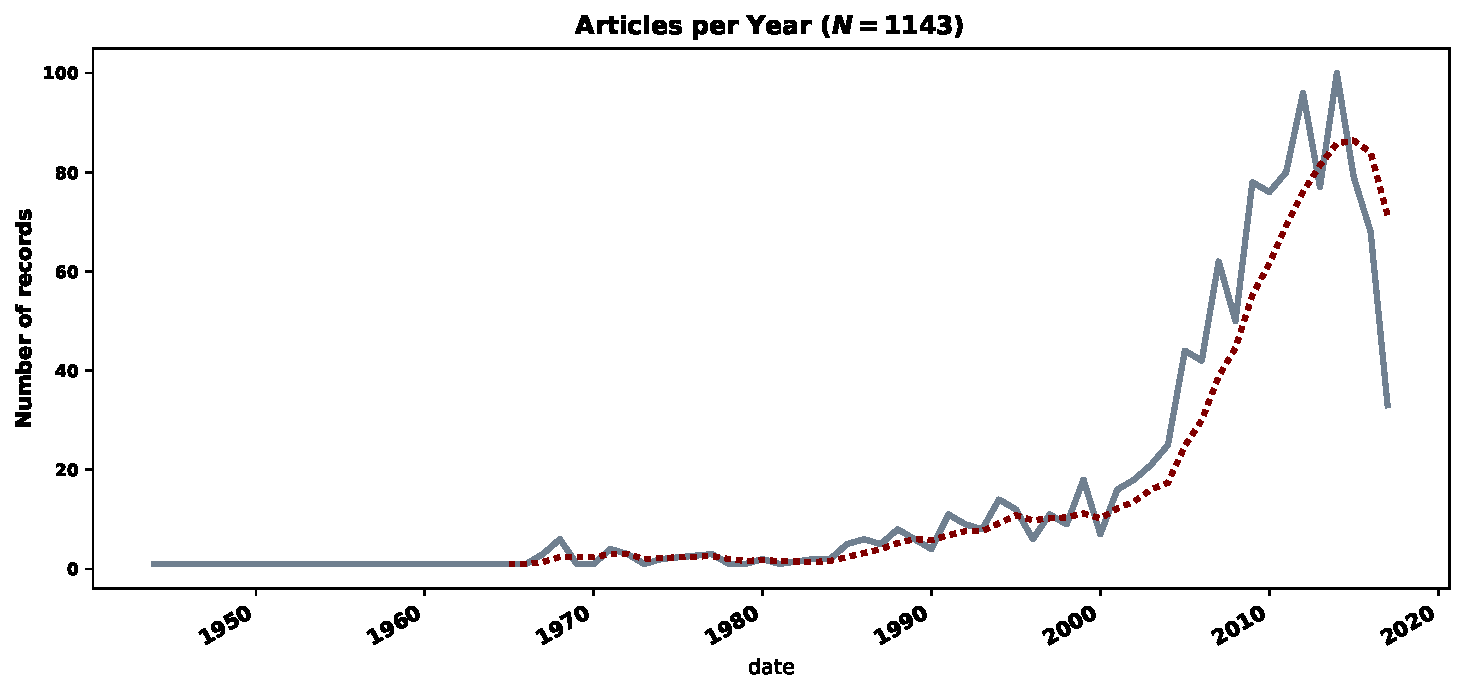
\includegraphics[width=0.6\textwidth]{./assets/images/timeseries.pdf}
    \caption{Time series of main data set and the rolling average.}\label{fig:timeseries}
\end{figure}

\begin{table}[!hbtp]
    \begin{center}
    \begin{tabular}{lr}
\toprule
{} &   Forecast \\
\midrule
1  &  27.301817 \\
2  &  24.500512 \\
3  &  26.490962 \\
4  &  26.208756 \\
5  &  27.004436 \\
6  &  27.288891 \\
7  &  27.815812 \\
8  &  28.227735 \\
9  &  28.694200 \\
10 &  29.134797 \\
\bottomrule
\end{tabular}

    \end{center}
    \caption{Forecasting the number of publications over the next 10 years.}
    \label{table:forecast}
\end{table}

Thought the time series has indicated a slight decrease we can see that the
model forecasts an increase over the next years.

\subsubsection{Auction games and the price of anarchy data sets}

Two subfields of game theory are chosen for this work; auction game and the
price of anarchy. A summary of both data sets collected on this two topics %TODO: cite
is given by Table~\ref{table:summary_other_topics}.

A total of 2103 articles with 3860 unique authors are examined for auction games.
Auction games is well studied topic with the earliest entry going
back to 1974. In comparison, 296 unique articles have been collected on price of
anarchy. The earliest entry being in 2003 and a total of 668 unique authors have
written about the topic.

In Figure~\ref{fig:timeplots_other_topics} a time plot for each topic is
displayed and is exhibited that both topics have had an increasing trend over
the years. Though price of anarchy is clearly a new topic compared to auction games.

The frequency of the prisoner's dilemma, for both articles and authors, lies
between the frequencies of these two topics.

\begin{table}[!hbtp]
    \begin{center}
    \begin{tabular}{llr}
        \toprule
         &            Price of anarchy &  Auction games \\
        \midrule
        Unique articles      & 296  & 2103 \\
        Unique authors       & 668  & 3860 \\
        Min publication year & 2003 & 1974 \\
        Max publication year & 2017 & 2017 \\
        \bottomrule
    \end{tabular}
    \end{center}
    \caption{Secondary data sets summaries.}
    \label{table:summary_other_topics}
\end{table}

\begin{center}
\begin{figure}[!hbtp]
    \begin{subfigure}{0.5\textwidth}
        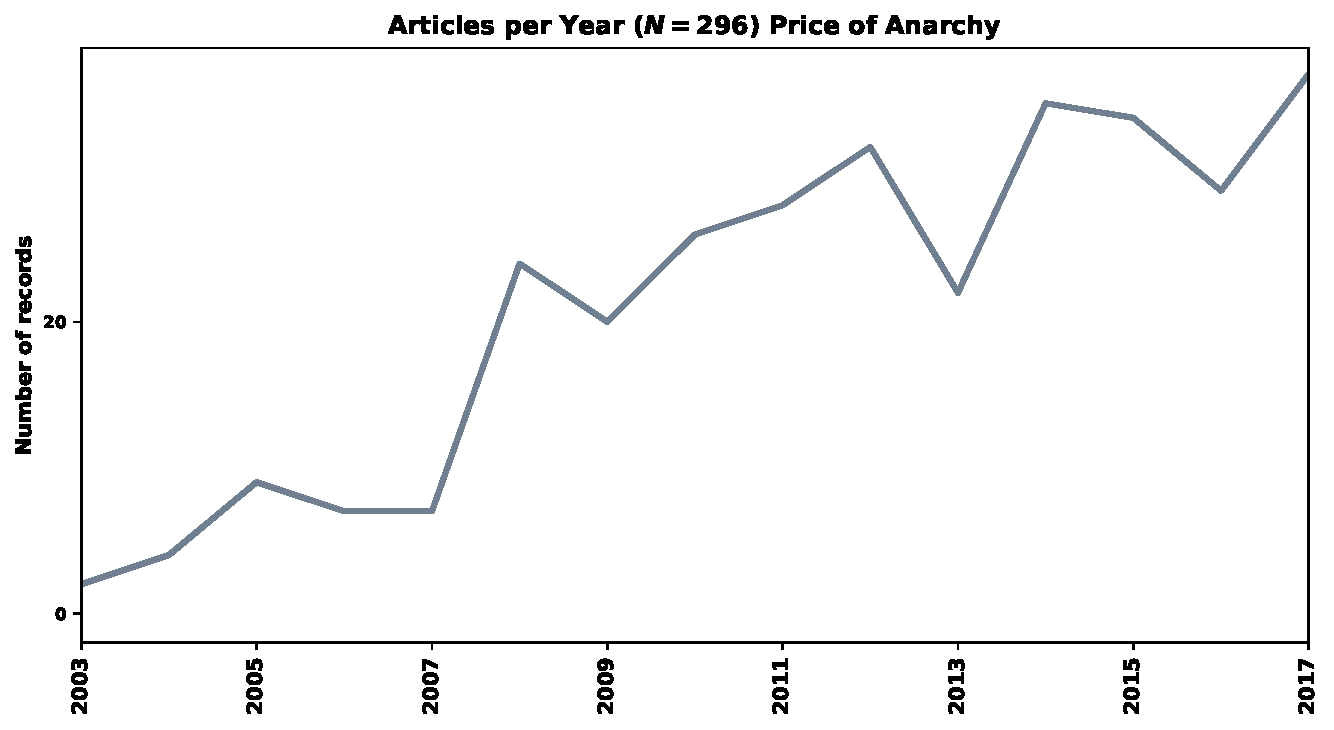
\includegraphics[width=\textwidth]{./assets/images/anarchy_timeline.pdf}
    \end{subfigure}
    \begin{subfigure}{0.5\textwidth}
        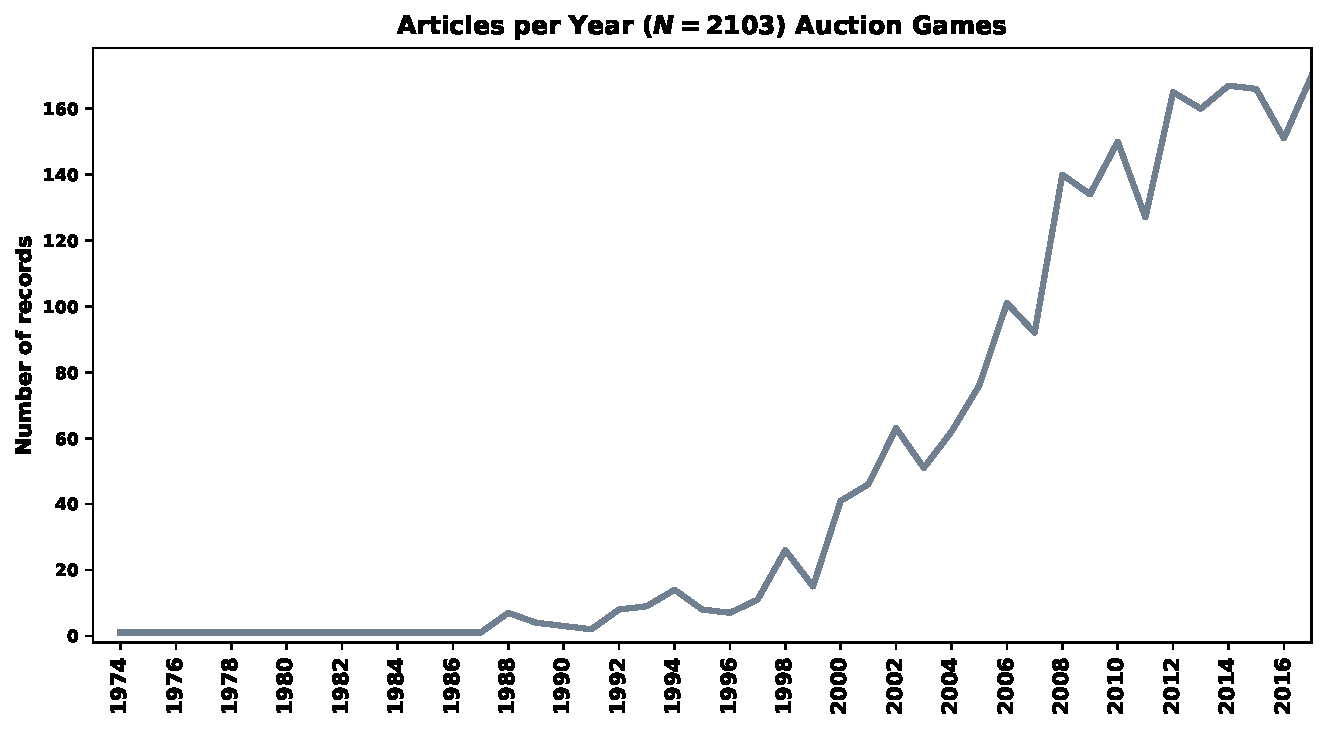
\includegraphics[width=\textwidth]{./assets/images/auction_timeline.pdf}
    \end{subfigure}
\caption{Time plots for secondary data sets.} % TODO cite
\label{fig:timeplots_other_topics}
\end{figure}
\end{center}

The provenance of the articles is given by Table~\ref{table:provenance_other_topics}.
Almost 1500 article for auction games have been collected from Springer, that is
more than three times the articles that have been collected from other sources.
PLOS and Nature have a minor contribution and PLOS and Nature had no
articles on the price of anarchy.

\begin{table}[!hbtp]
    \begin{center}
    \begin{tabular}{lcc}
        \toprule
        \textbf{Provenance} & \textbf{Total articles} & \textbf{Total articles}\\
                   & (auction games) & (price of anarchy)\\
        \midrule
        Springer   &                1429 &                78 \\
        arXiv      &                 436 &                108 \\
        IEEE       &                 301 &                131 \\
        PLOS       &                  15 &                 -  \\
        Nature     &                   1 &                 -   \\
        \bottomrule
    \end{tabular}
    \end{center}
    \caption{Articles' provenance for secondary data sets.}
    \label{table:provenance_other_topics}
\end{table}

\begin{table}[!hbtp]
    \begin{center}
    \begin{tabular}{lcc}
        \toprule
        \textbf{Provenance} & \textbf{Av. publication}  & \textbf{Av. publication}\\
                            & (auction games) & (price of anarchy)\\
        \midrule
        Overall             &          58.973 & 19.812 \\
        Springer            &          38.622 & 4.875  \\
        arXiv               &          11.784 & 6.750   \\
        IEEE                &           8.135 & 8.188    \\
        PLOS                &           0.405 &   -       \\
        Nature              &           0.027 &   -        \\
        \bottomrule
    \end{tabular}
    \end{center}
    \caption{Average publication for auction games and the price of anarchy.}
    \label{table:other_topics_publication_rates}
\end{table}

The overall average publication for auction games and the price of anarchy are 59 and 20 articles
respectively. It appears that auction games publication is largely different
for both the prisoner's dilemma and the price of anarchy. These two topics have
the same average publication. Note that the significance of each journal differs
from topic to topic. Though this analysis will not focus on individual sources
from hereupon.

% \paragraph{Temporal analysis}
% \mbox{ }\\

% For comparison reasons in the following subsections the analysis will also be
% held relative to a temporal analysis. The main data set~\cite{}
% is divided into time period according to the subsections of Section~\ref{section:timeline}.
% The respective measures of unique titles and unique authors for each period is
% given by Table~\ref{table:summary_temporal}.

% \begin{table}[!hbtp]
%     \begin{center}
%     \begin{tabular}{lrr}
\toprule
{} &  \textbf{Unique articles} &  \textbf{Unique authors} \\
\midrule
period 1: (1961 - 1972) &               21 &              38 \\
period 2: (1981 - 1984) &                5 &               6 \\
period 3: (1984 - 1993) &               64 &              70 \\
period 4: (1987 - 1999) &              121 &             169 \\
period 5: (1995 - 2015) &              926 &            1730 \\
period 6: (2012 - 2017) &              453 &            1008 \\
period 7: (2015 - 2017) &              180 &             466 \\
\bottomrule
\end{tabular}

%     \end{center}
%     \caption{Periods and their respective measures.}
%     \label{table:summary_temporal}
% \end{table}

In this section we have described the three data sets that we are going to use
in the following sections in order to identify collaborative behaviour and influence.
Two data sets of different topics are used for comparison reasons. The frequency of
articles and authors differs within the three data sets which is ideal.
% Finally a temporal analysis of the data sets~\cite{} will also assists us in
% obtaining more insights. The period have also be presented here.


\subsection{Co authorship Analysis}\label{section:co_authorship_analysis}

Most academic research is undertaken in the form of
collaborative effort. As discussed in~\cite{Kyvik2017}, it is rationale that two
or more people have the potential to do better as a group than individually. Academic collaborations
have many different forms. Researchers might have immediately collaborated and
written together. Others might have collaborated through a common co author.

Collaboration in groups has a long tradition in experimental sciences and it has
be proven to be productive according to~\cite{Etzkowitz1992}. Even so, the number of collaborations
can be very different between research fields and measuring collaboration is
not always an easy task. Another aspect of collaborative behaviour is influence. For
example academics can influence through workshops, talks or by collaborating with people
in our environment.

Several studies tend to consider academic citations as a measure for these things.
As discussed in~\cite{nature_blog}, depending on citations can often be misleading.
This is because:

\begin{itemize}
    \item The true number of citations can not be known. Citations can be missed
    due to data entry errors.
    \item Academics are influenced by many more papers than they actually cite.
    \item Several citations are superficial.
\end{itemize}

We suggest an alternative measure of collaboration and influence by looking at the co
authorship network. A co authorship network,
is a network where academics that have written and published together are connected.

Using graph theoretic concepts this network will be analysed to undestand:

\begin{itemize}
    \item Collaborativeness; for example the number of connections an author has
    as well as more sophisticated measures of closeness.
    \item Influence; how many connections are made possible because of an author.
\end{itemize}

We introduced several network measures that we will be using such as:

\begin{itemize}
    \item Number of connected components.
    \item Clustering coefficient.
    \item Degree distributions.
    \item Centrality.
\end{itemize}

\subsubsection{Constructing a co authorship network}

To construct a co authorship network we need to consider all the unique authors.
The issue with retrieving the unique authors is that authors names can be written
in different ways in different sources. For example consider the author of this
paper:

\begin{itemize}
    \item Nikoleta Glynatsi
    \item Nikoleta E. Glynatsi
    \item Nikoleta Evdokia Glynatsi
\end{itemize}

Consequently, several different entries of the same author existed within the data
set. Thus we wanted to figure out when two author names were the same in real life.
Though identifying if two string correspond to the same author is human possible
the data sets consited of more than 1000 authors, thus we wanted to automate the
procedure.

This was done by using the Levenshtein Distance~\cite{miller2009}. The Levenshtein
Distance is a metric for measuring the difference between two sequences. It is
based upon the number of actions one has to take to transform one string into
the other. These actions include:

\begin{enumerate}
    \item Insertion;
    \item Deletion;
    \item Substitution of a single character.
\end{enumerate}

Let us consider an example where we are trying to calculate the distance between
the two strings. These are `Wang' and `Yang'. To compute the distance in a non-recursive
way, we use a matrix \(D\) containing the distances between all the prefixes of the
two strings. The first row and column are indexed by empty strings. The rest of
the rows and columns are index by the prefixes of the two strings.

The matrix is filled from left to right. The first row is filled as follows:

\begin{enumerate}
    \item To go from an empty string to an empty string zero actions are needed.
    Thus the \(D_{\text{e}, \text{e}}\) is 0.
    \item To go from an empty string to `W', or the other way around, 1 action
    is needed. Thus the \(D_{\text{e}, \text{W}}\) is 1.
    \item For every new letter we have to take another action \((+1)\).
\end{enumerate}

Similarly, this is done for the first columns. For rest of the elements
we follow a similar approach, but this time the previous distances are also
taken in account. For example, \(D_{\text{Y}, \text{W}}\). For the letter `Y'
to go to `W' a single action is required. Note that now 1 is added to the minimum
distance between of \(D_{\text{e}, \text{e}}, D_{\text{e}, \text{W}}\) and
\(D_{\text{e}, \text{Y}}\). 

Similarly we fill the rest of matrix. The last value computed, bottom right,
is the Levenshtein Distance of the two strings. In our example it is calculated
to be 1.

\[ D = \kbordermatrix{
     & \text{e} & \text{W} & \text{A} & \text{N} & \text{G} \\
   \text{e} & 0 & 1 & 2 & 3 & 4 \\
    \text{Y} & 1 & 1 & 2 & 3 & 4 \\
    \text{A} & 2 & 2 & 1 & 2 & 3 \\
    \text{N} & 3 & 3 & 2 & 1 & 2 \\
    \text{G} & 4 & 4 & 3 & 2 & 1
  }\]

In this work we calculate the ratio of two string matching for all possible
pairs of authors in the data sets. The matching ratio is calculated as,

\[(1 - \frac{\text{lev}}{m}) \times 100,\]

where \(\text{lev}\) is the distance and \(m\) is the length of the longest of
the two words. If the ratio of a pair was between \(85\) and \(99\) both entries
were highlighted. The highlighted entries were manually checked to assure that
there were indeed the same author and then one of them was replaced by the other.

For example all entries with author name written as example ``Y. Moreno'' were
replaced by ``Yamir Moreno''.

The manual check is performed because not all highlighted entries are indeed the
same. For example:

\begin{enumerate}
    \item Zhen Yang and
    \item Zhen Wang
\end{enumerate}

are two different authors. Once the name entries have been cleaned the
co authorship networks can be defined. The definition of a co authorship network
is given by:

\begin{definition}{Co authorship network.}
    A co authorship network is an undirected network \(G\) of vertices \(V\) and
    edges \(E\) where vertices representing each unique author and an edge
    connects two authors if and only if those authors have written together.
    No weight has been applied to the edges nor the nodes.
\end{definition}

%Define what a network is and then G_1, G_2, G_3
The three networks considered:

\begin{itemize}
    \item \(G_1\), the prisoner's dilemma network, where \(V(G_1)=\) \authors and
    \(E(G_1)=\) \edges.
    \item \(G_2\), the auction games network, where \(V(G_2)=\) \auctionauthors and
    \(E(G_2)=\) \auctionedges.
    \item \(G_3\), the auction games network, where \(V(G_3)=\) \priceauthors and
    \(E(G_3)=\) \priceedges.
\end{itemize}

The respective illustrations of \(G_1, G_2\) and \(G_3\) are given by Figures
\ref{fig:authors_network} and \ref{fig:co-authorship-other-topics}.

\begin{figure}[!hbtp]
    \centering
    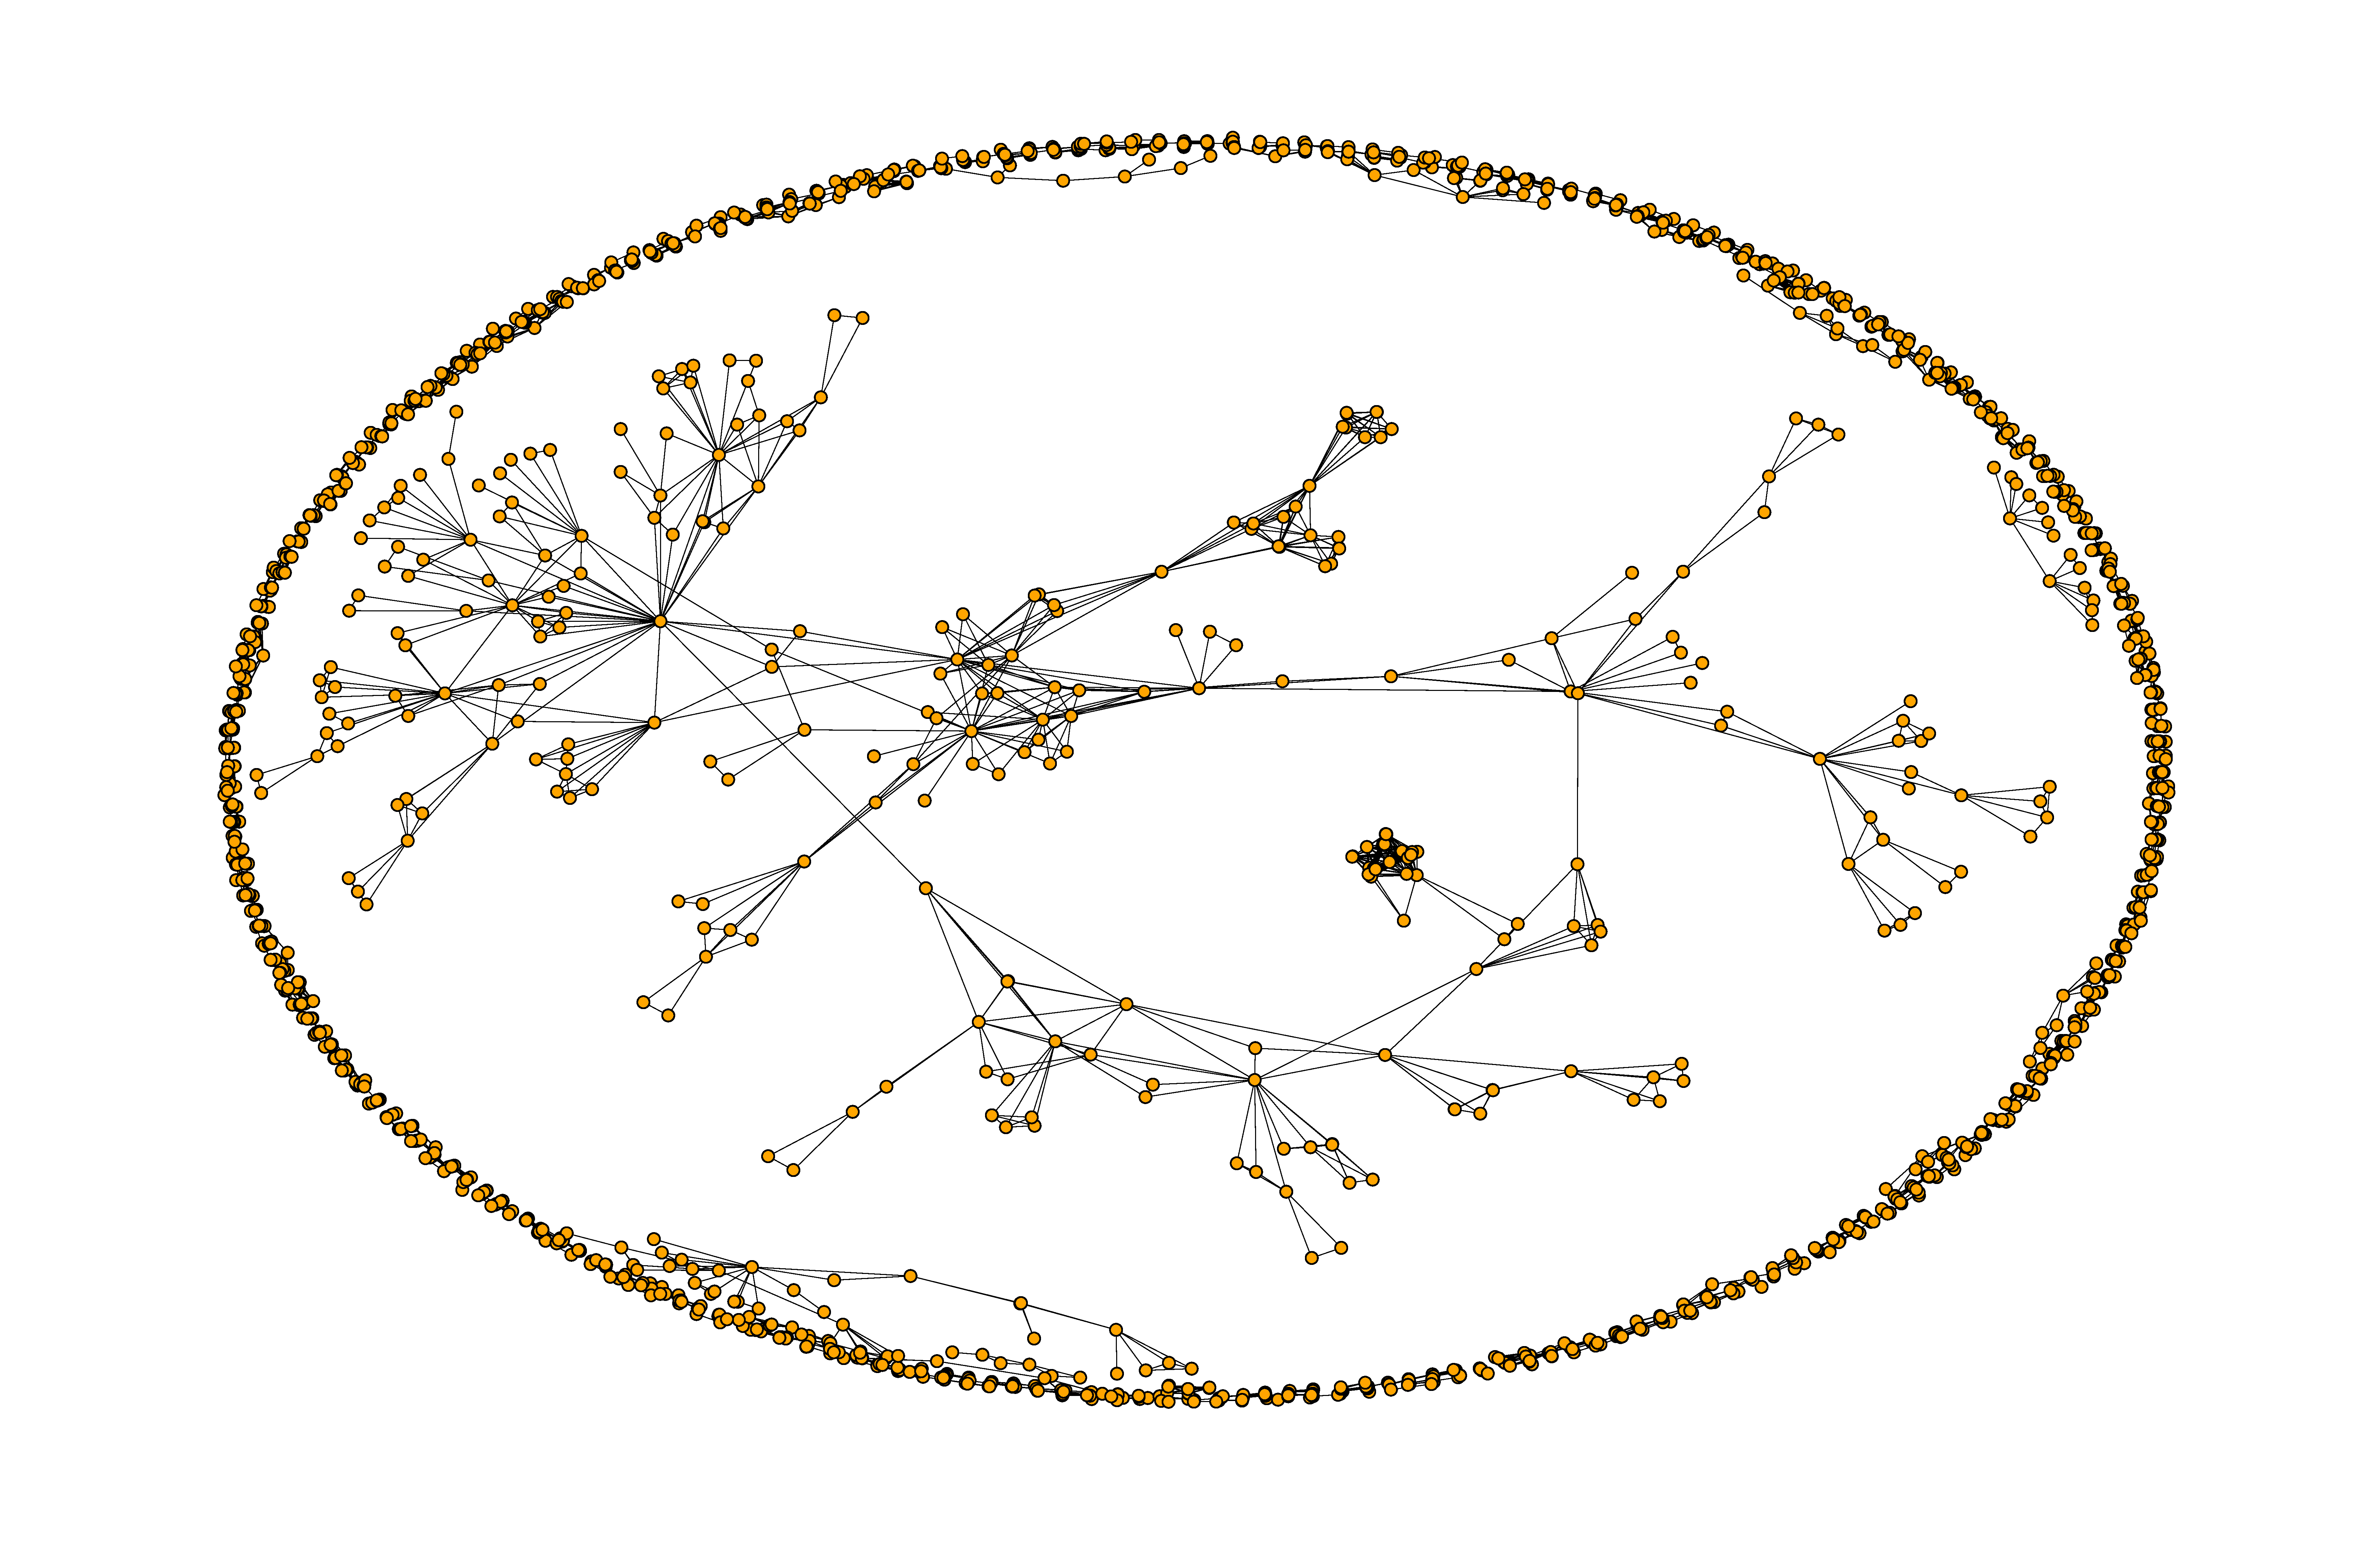
\includegraphics[width=0.8\textwidth]{./assets/images/co-authors-network.pdf}
    \caption{Co authorship network for the prisoner's dilemma.}\label{fig:authors_network}
\end{figure}

\begin{center}
    \begin{figure}[!hbtp]
        \begin{subfigure}{0.5\textwidth}
            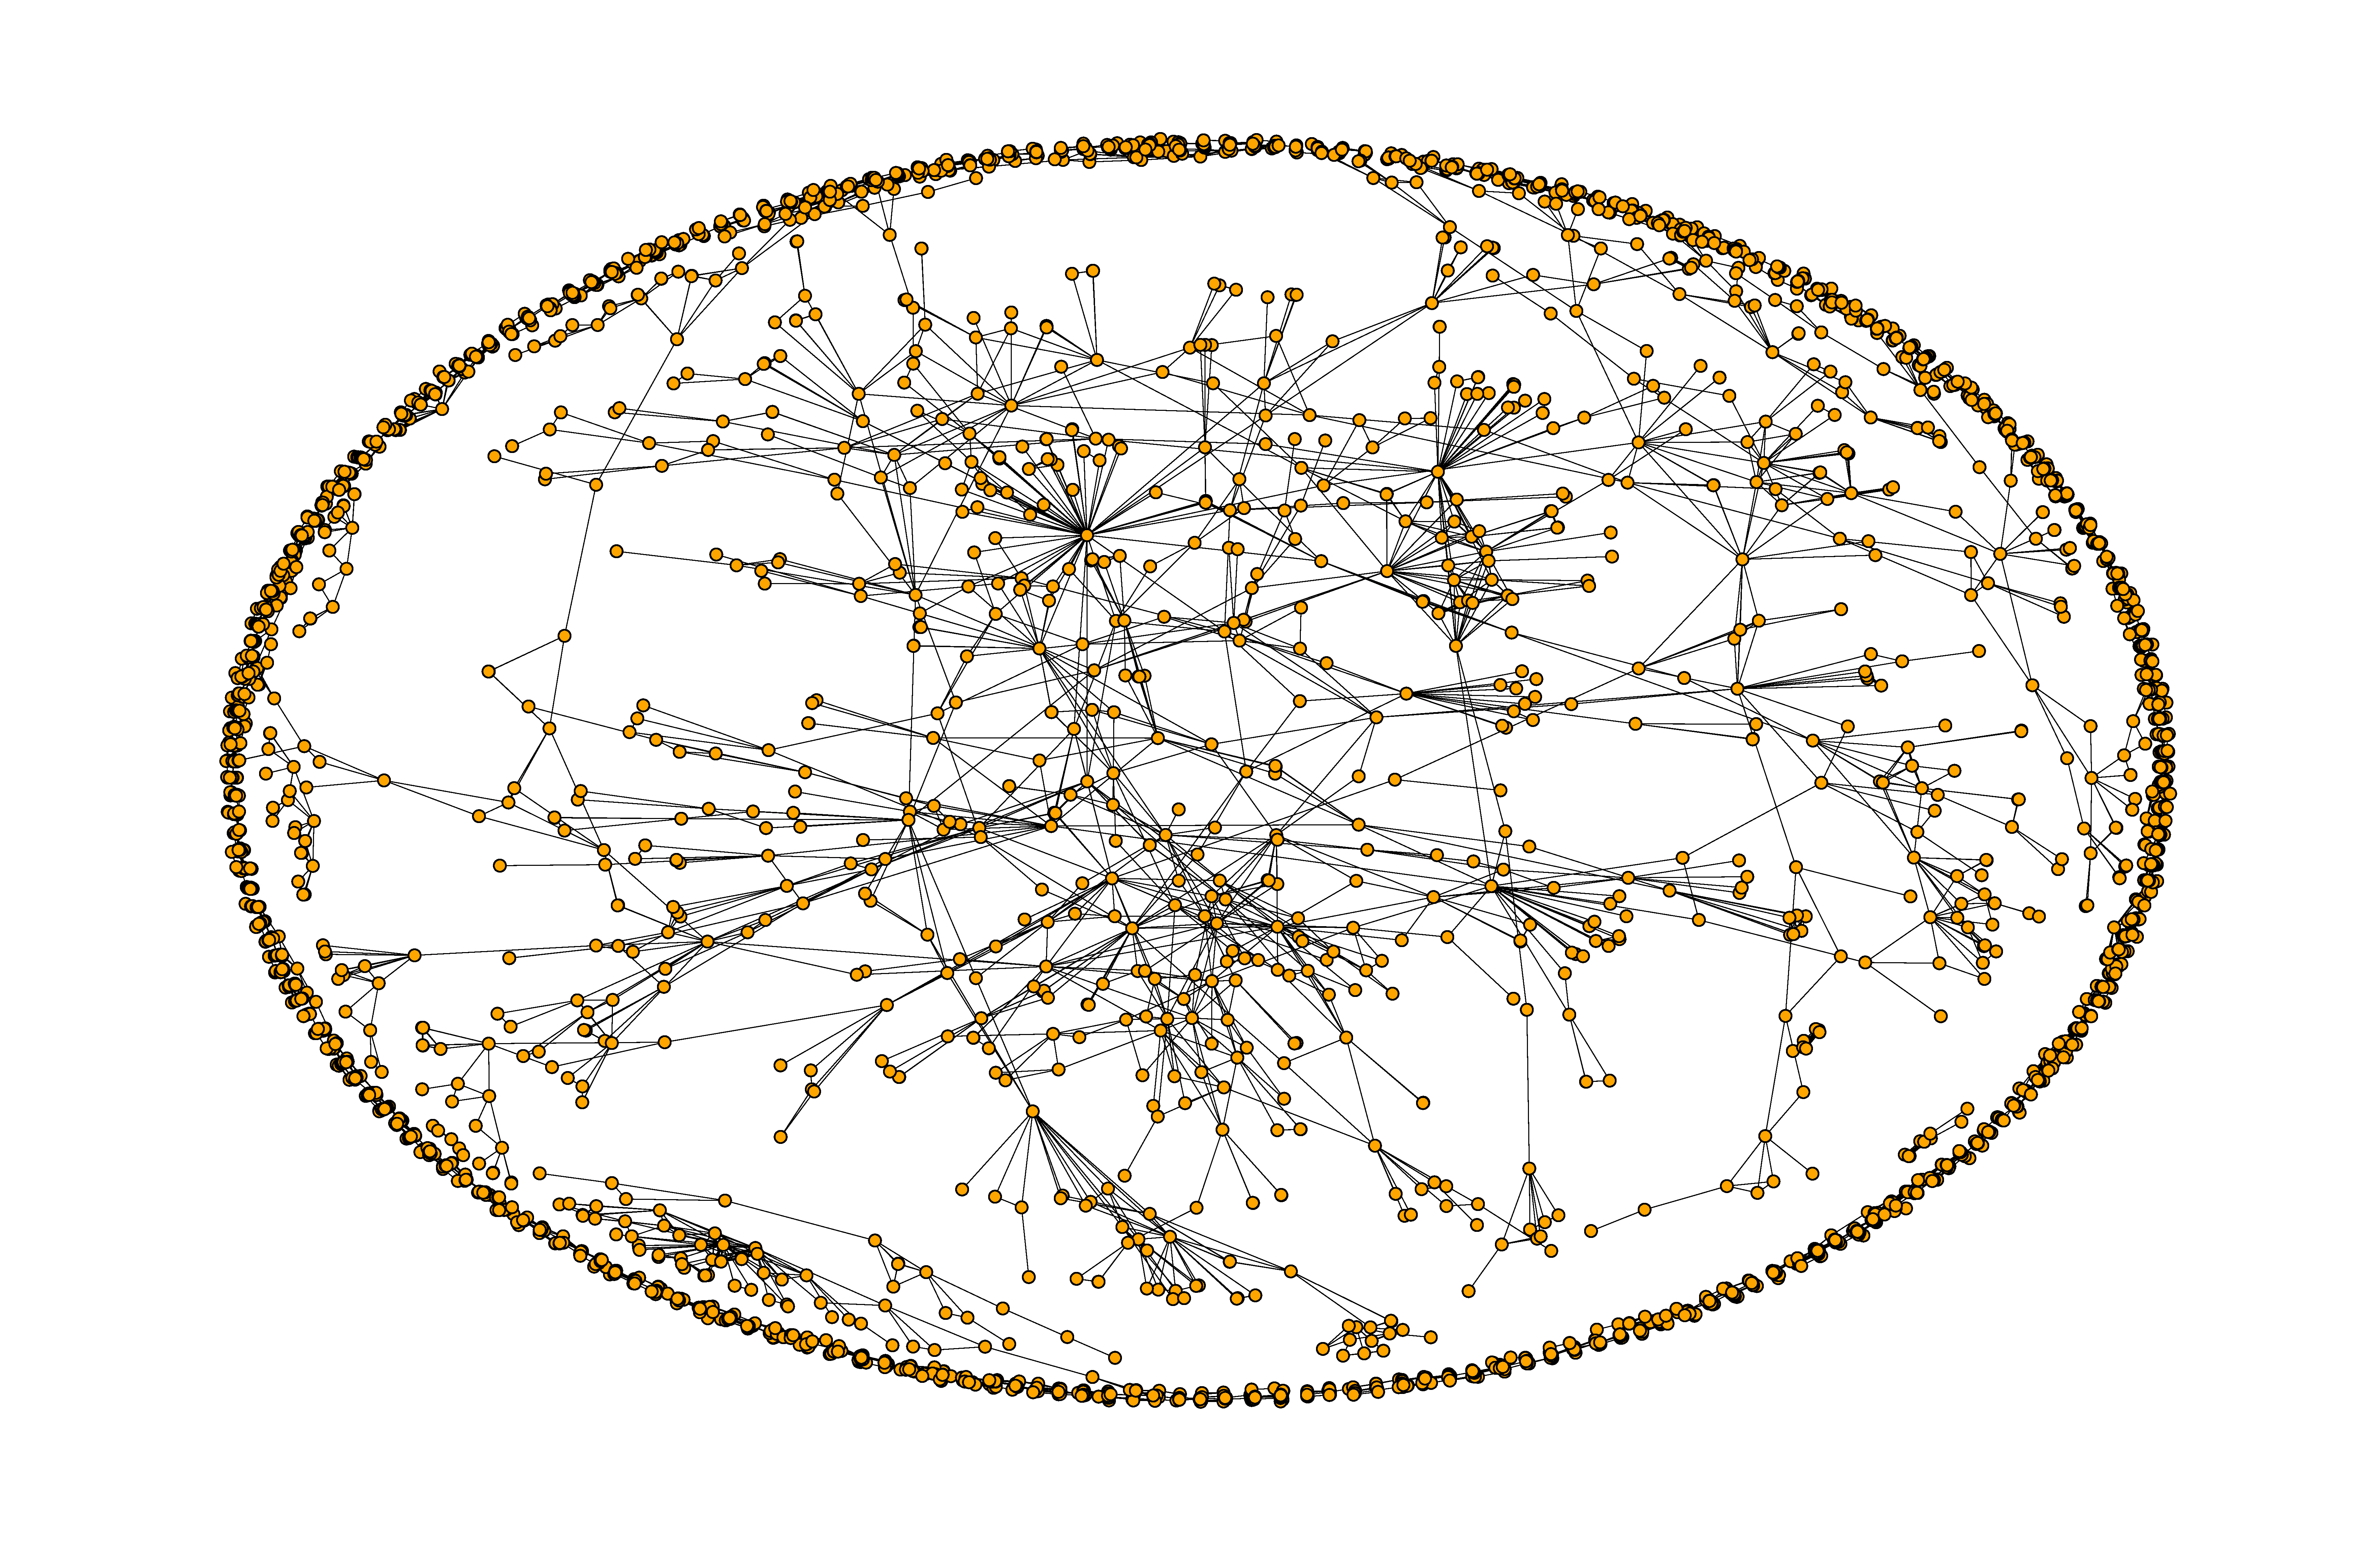
\includegraphics[width=\textwidth]{./assets/images/co-authors-network-auction.pdf}
            \caption{Co authorship network for auction games.}
        \end{subfigure}
        \begin{subfigure}{0.5\textwidth}
            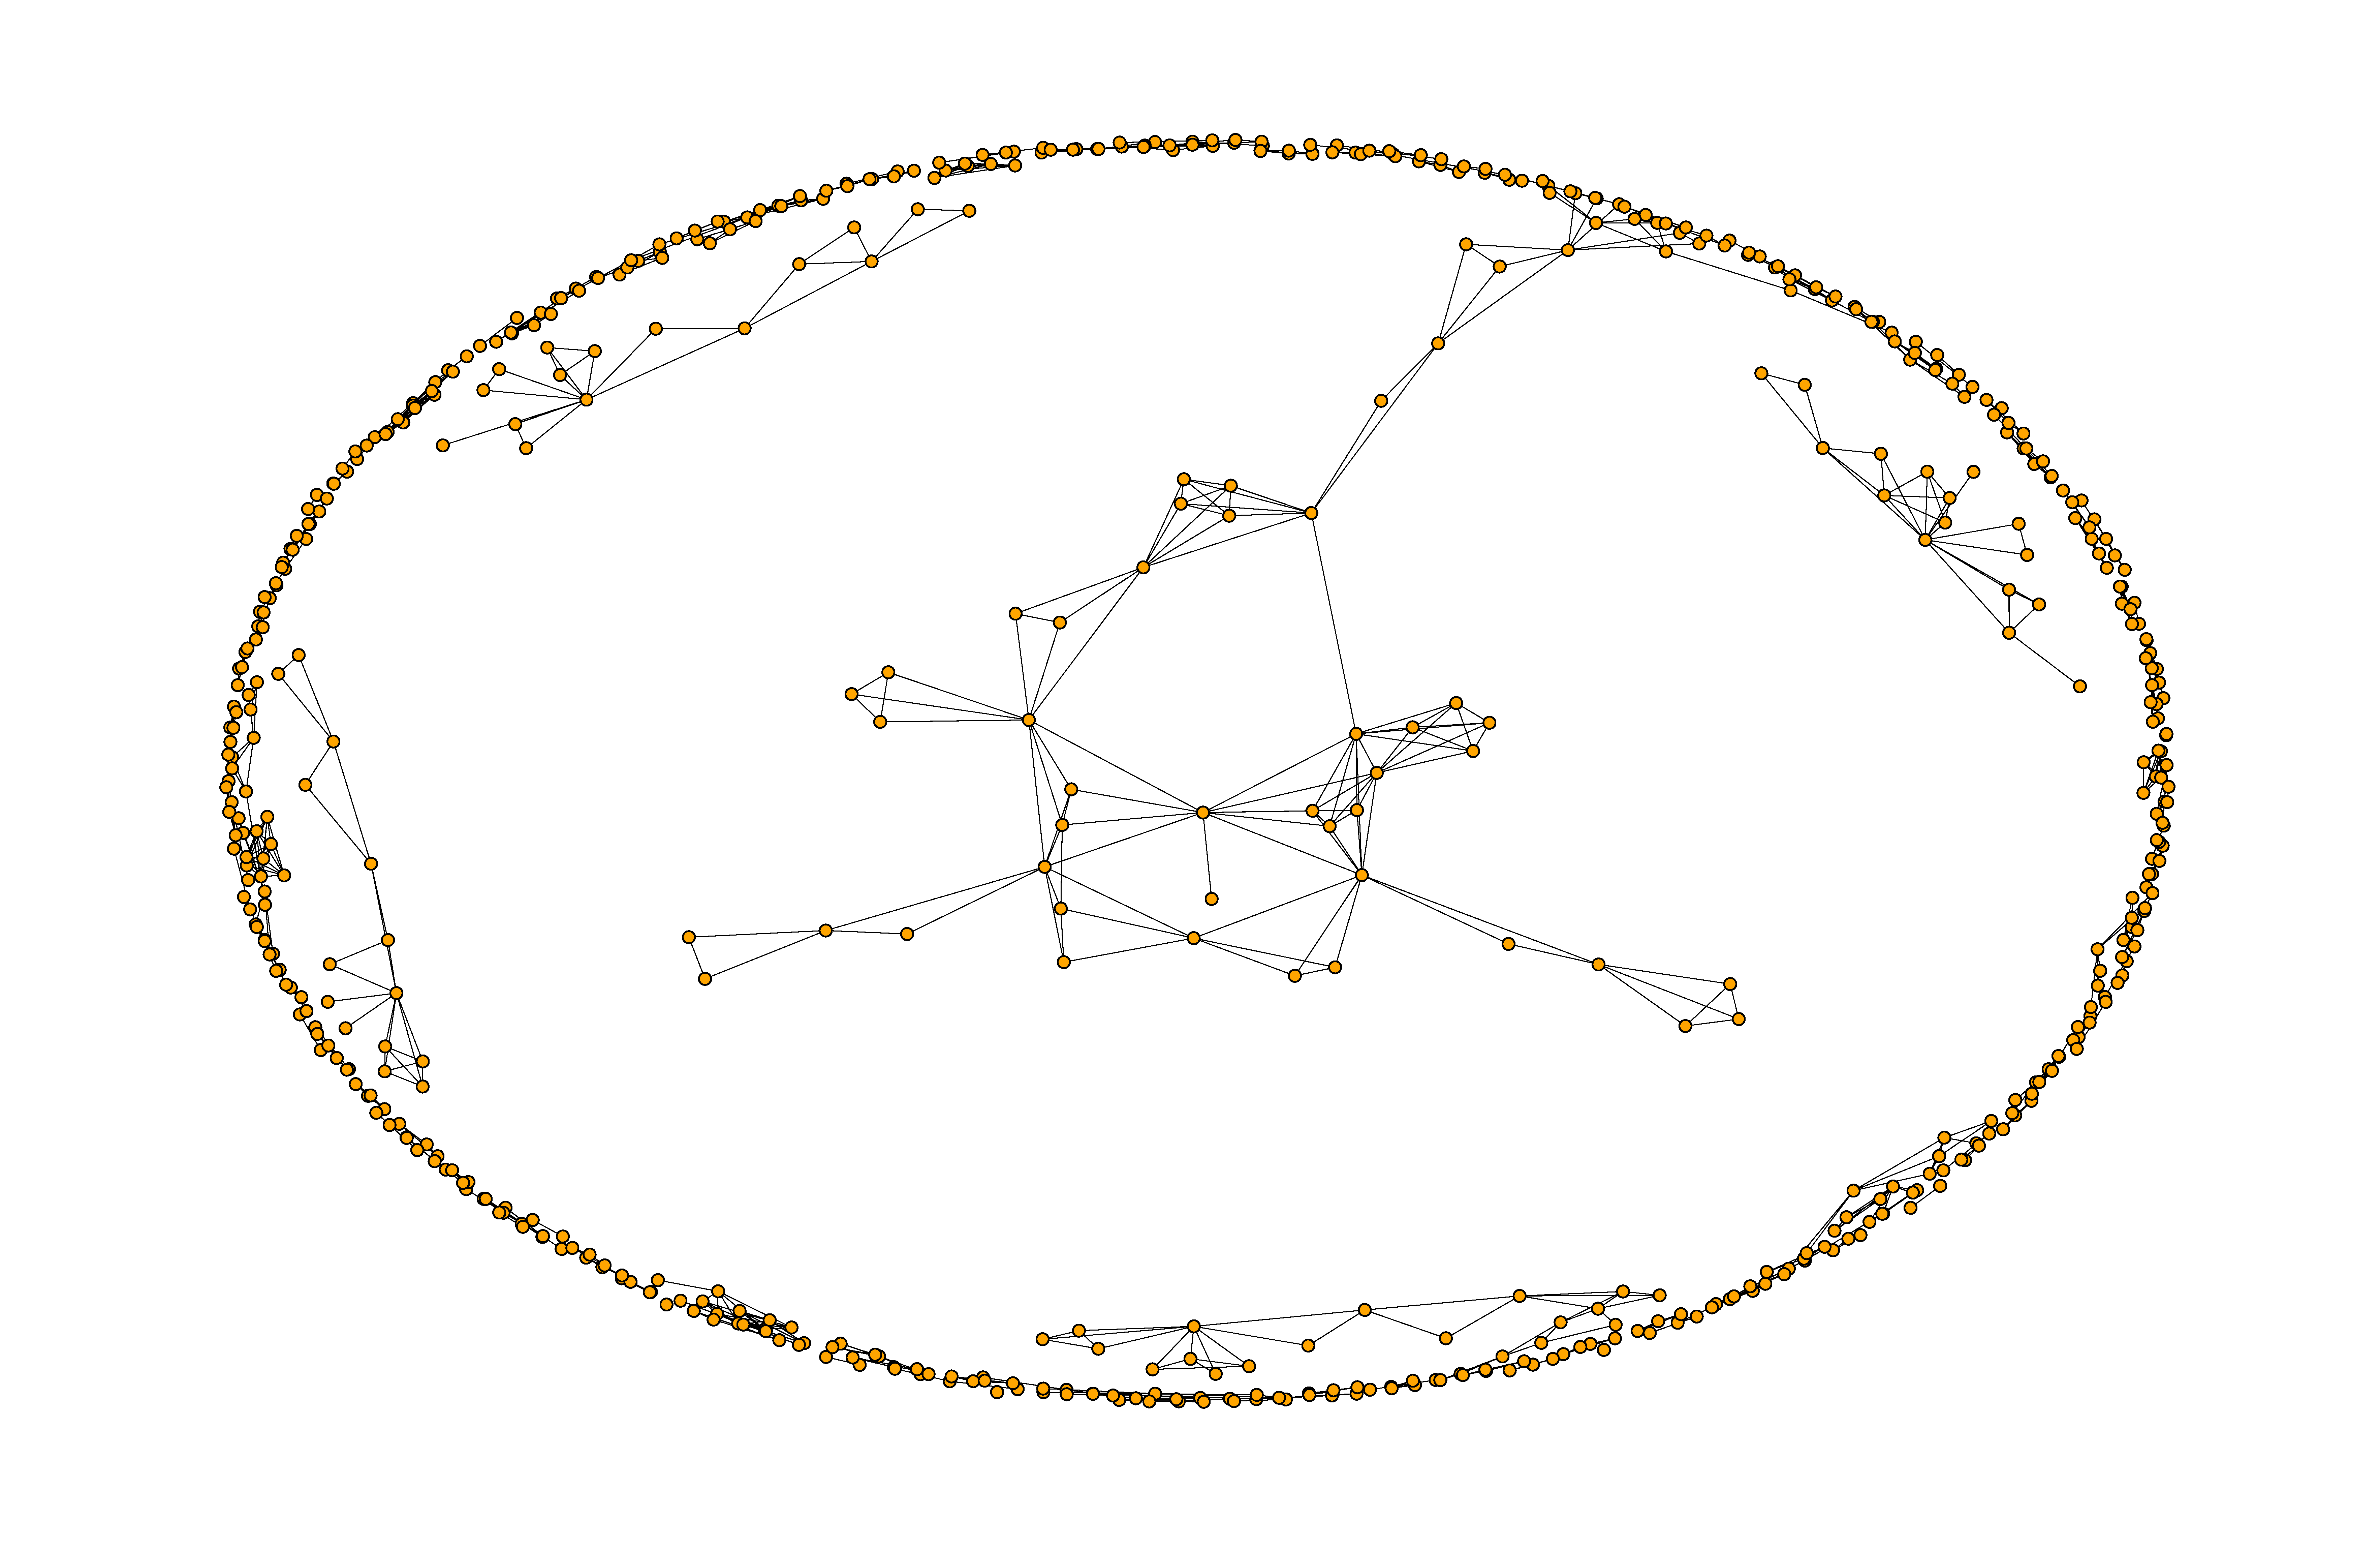
\includegraphics[width=\textwidth]{./assets/images/co-authors-network-price.pdf}
            \caption{Co authorship network for the price of anarchy.}
        \end{subfigure}
    \caption{Co authorship network for secondary data sets.}
    \label{fig:co-authorship-other-topics}
    \end{figure}
    \end{center}

\subsubsection{Measures of collaboration}

In this section we ascertain the level of collaborative nature of the field.
This is measured as the connections authors can
have within their groups. Moreover, how strongly connected these groups are.
Several connectivity measures will be used to explain such behaviour which are
introduced through various examples.

The first measure introduced is the \textbf{number of connected components}. A connected
component of an undirected graph is a maximal set of nodes such that each pair
of nodes is connected by a path. Two examples are illustrated in Figure
\ref{fig:connected_components}. These are two different sub graphs of \(G_1\)
with a number of connected components of 1 and 5.

\begin{center}
\begin{figure}[!hbtp]
    \begin{subfigure}{0.5\textwidth}
        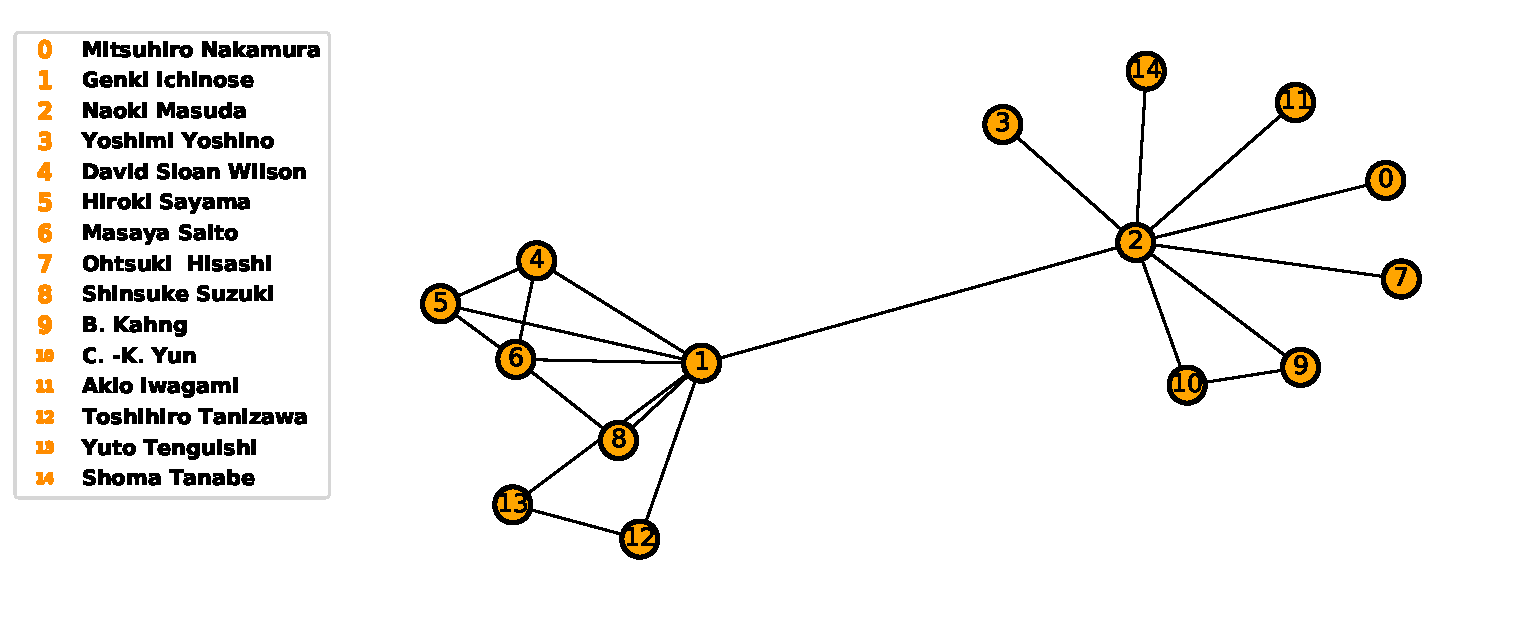
\includegraphics[width=\textwidth]{./assets/images/connected_example_one.pdf}
        \caption{A sub graph of \(G_1\) with 1 connected component.}
    \end{subfigure}
    \begin{subfigure}{0.5\textwidth}
        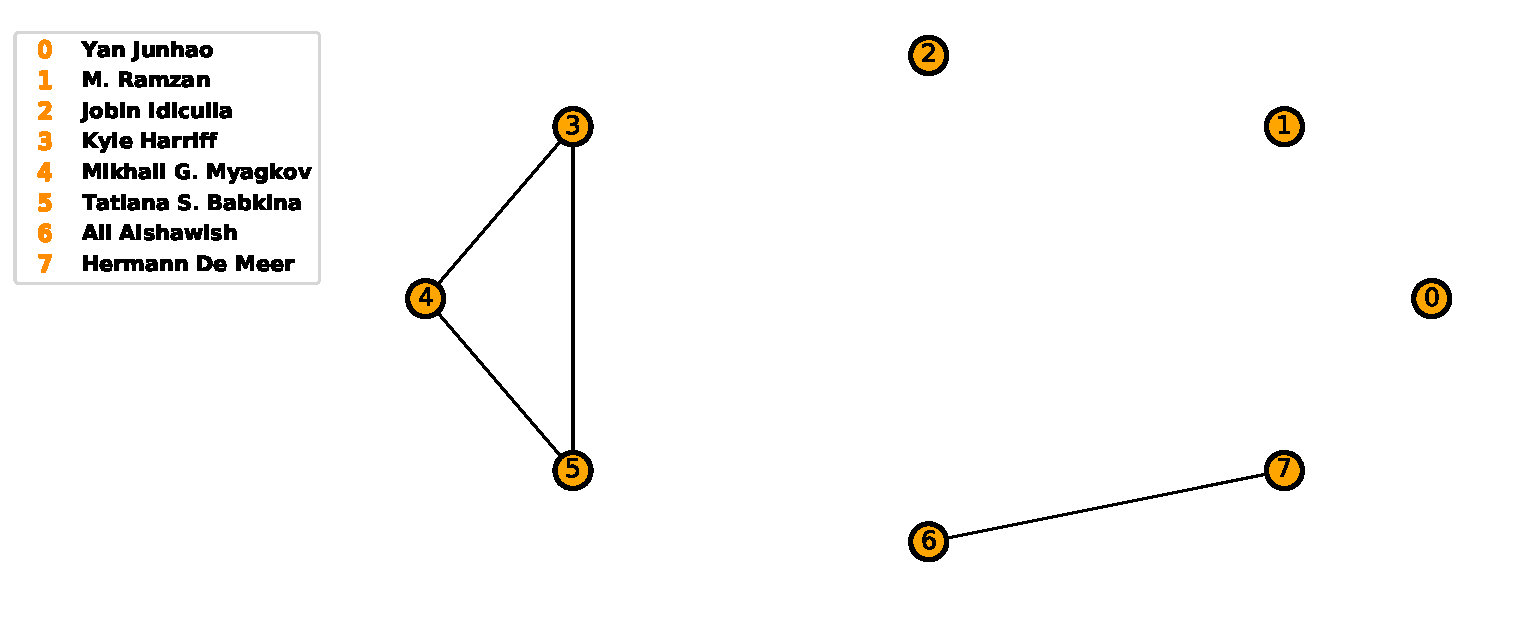
\includegraphics[width=\textwidth]{./assets/images/connected_example_two.pdf}
        \caption{A sub graph of \(G_1\) with 5 connected component.}
    \end{subfigure}
\caption{Connected components examples.}
\label{fig:connected_components}
\end{figure}
\end{center}

Note that a vertex with no incident edges is itself a connected component.
The number of connected components gives a naive measure of how disjoint the network is.
In essence the number of groups in the field.

The second measure considered is the \textbf{degree}. The degree of a node express
the number of connections a node has. We will consider the degree distribution
of a network. It will allow us to understand the mean connection that authors
have in the network's groups.

The final measure is the \textbf{clustering coefficient}. The clustering coefficient is a
measure of the degree to which nodes in a graph tend to cluster together. There
are two types of this measure; the local and the global coefficients. The local
coefficient is the clustering coefficient of a single vertex. It is calculated as,

\[C_u = \frac{2 \times L_u}{(k_u (k_u - 1)},\]

where \(k_u\) is the degree of vertex \(u\) and \(L_u\) is the number of edges
between \(k_u\) neighbours of vertex \(u\).

The global coefficient, \(\bar{C}\), is calculated by averaging all the local
coefficients of the graph. The values of the measure can range between \(0\) and
\(1\). Figure~\ref{fig:clustering_coefficients} illustrates several sub graphs
with different \(\bar{C}\) values.

\begin{center}
    \begin{figure}[!hbtp]
        \begin{subfigure}{0.33\textwidth}
            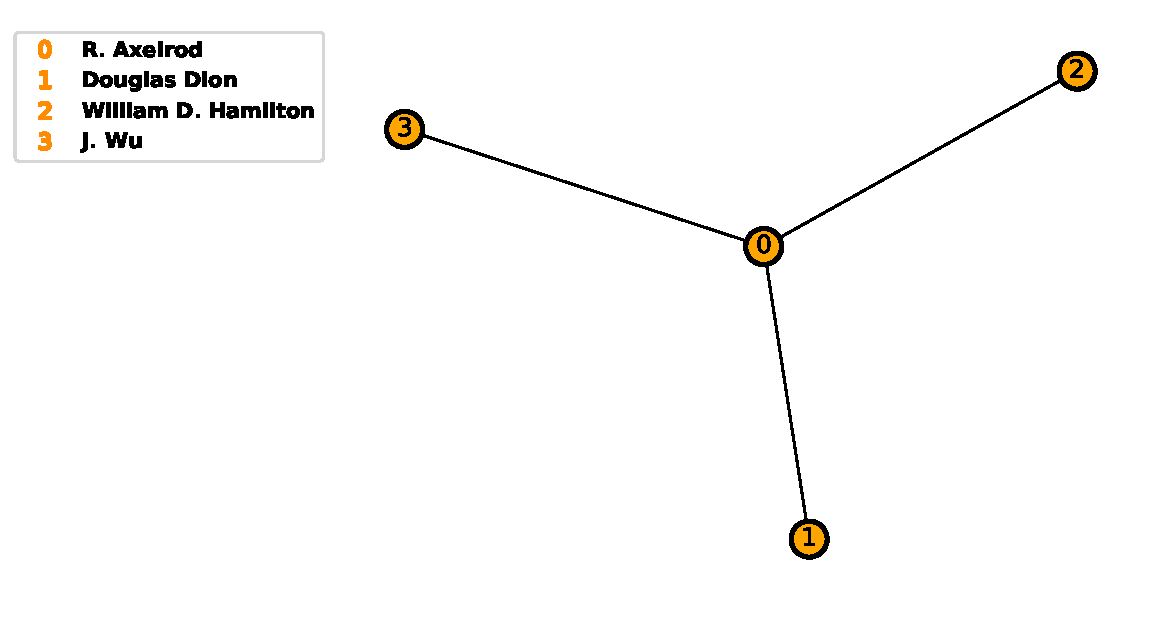
\includegraphics[width=\textwidth]{./assets/images/clustering_example_one.pdf}
            \caption{A sub graph of \(G_1\) with a global clustering coefficient of 0.}
        \end{subfigure}
        \begin{subfigure}{0.33\textwidth}
            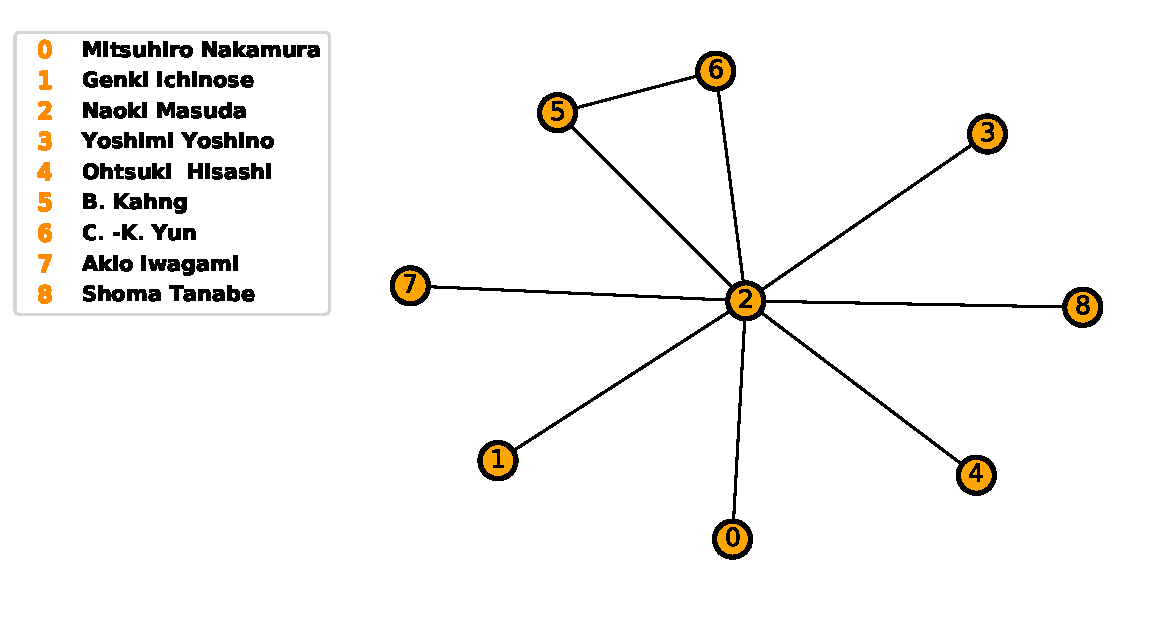
\includegraphics[width=\textwidth]{./assets/images/clustering_example_two.pdf}
            \caption{A sub graph of \(G_1\) with a global clustering coefficient of 0.23.}
        \end{subfigure}
        \begin{subfigure}{0.33\textwidth}
            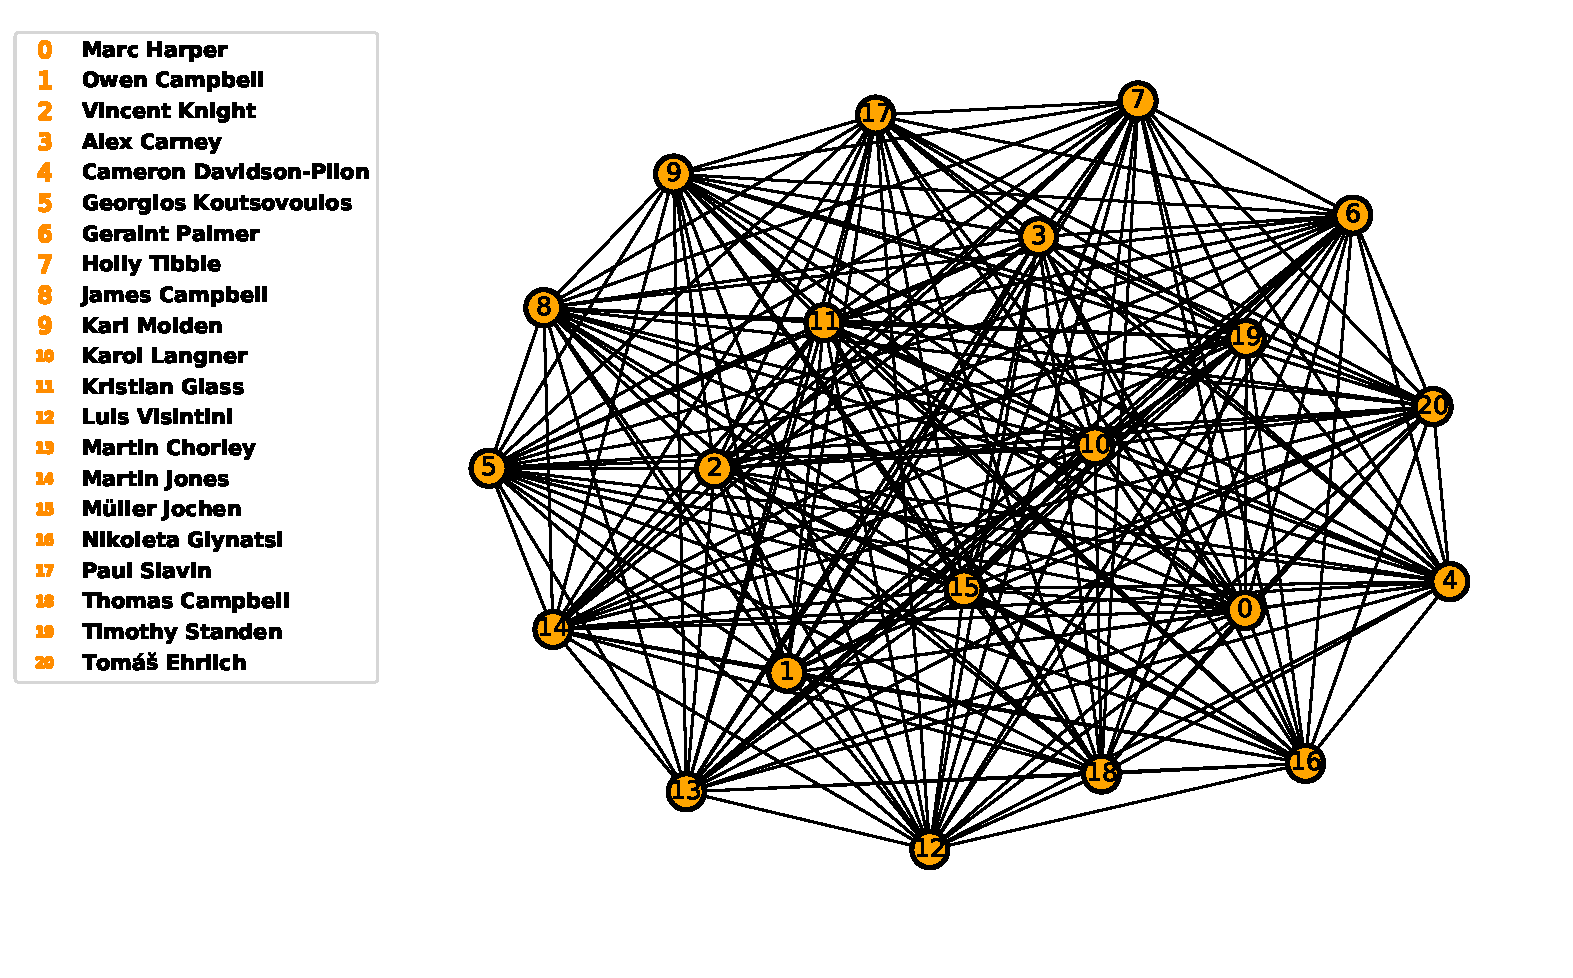
\includegraphics[width=\textwidth]{./assets/images/clustering_example_three.pdf}
            \caption{A sub graph of \(G_1\) with a global clustering coefficient of 1.}
        \end{subfigure}
    \caption{Clustering coefficients examples.}
    \label{fig:clustering_coefficients}
    \end{figure}
    \end{center}

A clustering coefficient of \(1\) indicates that a graph is a
complete graph. On the contrary, a coefficient of \(0\) indicates that authors write
with just a single co author.
% A high clustering coefficient indicates that people within groups have several
% connections. There are not there due to a single publication with a random researcher
% but on the contrary that group is said to be collaborative.

\paragraph{Analysis}
\mbox{ }\\

All connectivity measures are calculated for \(G_1, G_2\) and \(G_3\). This is
done using the open source package networkx~\cite{networkx}.

We are aware that all three of the networks are disjoint. This is also verified
by the number of connected components. More specifically there are \prisonerscon,
\auctioncon and \pricecon for graphs \(G_1, G_2\) and \(G_3\) respectively.
% Though the number of connected components for \(G_1\) is between \(G_2\) and \(G_3\)
% we believe that this could be due the size of the data sets.
% The of authors that have written by themselves was also calculated.
A total of \prisonerisolated, \auctionisolated, \priceisolated authors have
written by themselves, for graphs \(G_1, G_2\) and \(G_3\) respectively.

The normalised degree distributions of all three networks are shown in Figure~\ref{fig:degrees_dist}.
They have been normalised such that the frequencies sum to one. 
None of the distributions is normally distributed thus the non parametric test
Kruskal-Wallis is used~\cite{mckight2010}. Kruskal-Wallis allow us to compare the
medians of two or more distributions. The test returns a \(p\)-value of 0.29.
Thus there is significant difference at the level of 0.005.

\begin{figure}[!hbtp]
    \centering
    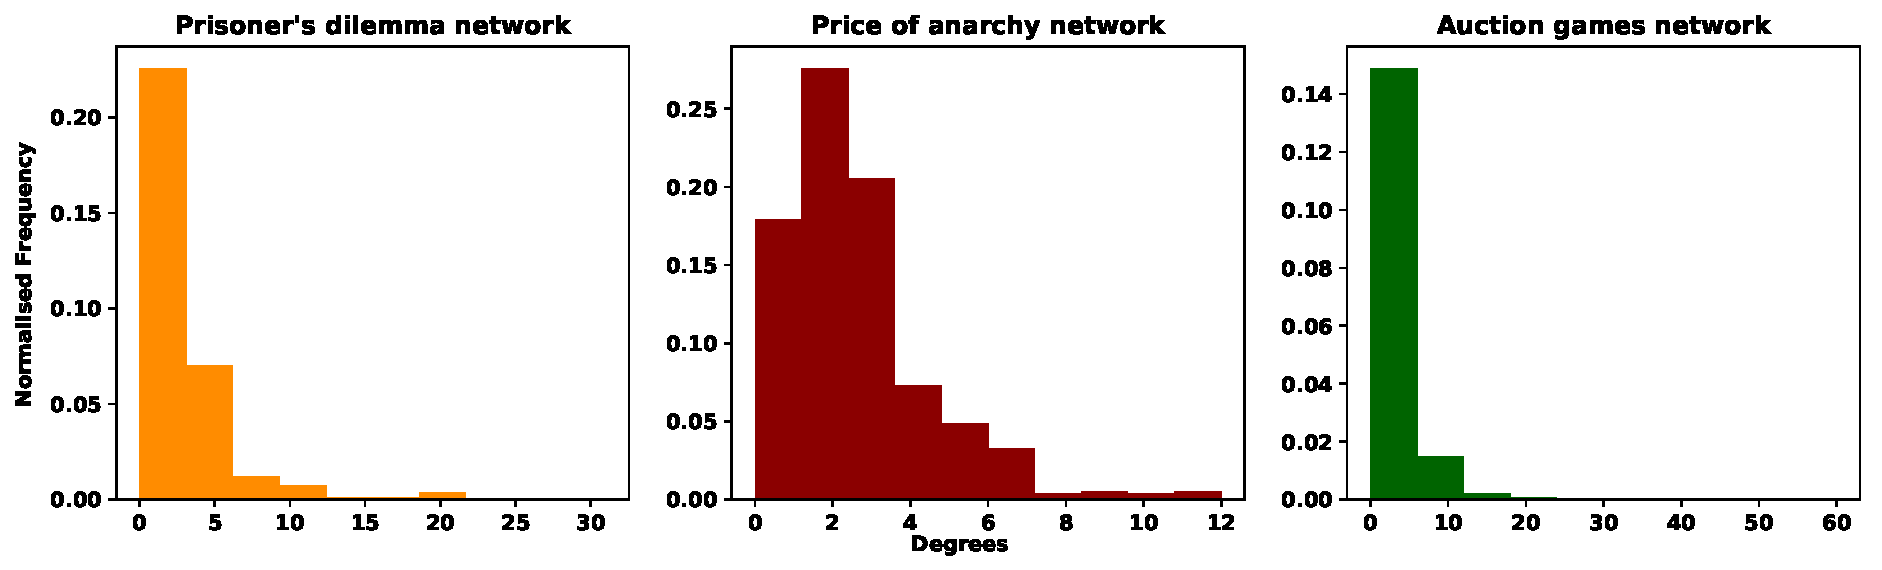
\includegraphics[width=\textwidth]{./assets/images/degrees_histrograms.pdf}
    \caption{Degree distributions for all three networks.}\label{fig:degrees_dist}
\end{figure}

The global clustering coefficients of all three networks are presented in Table
\ref{table:clustering}. The price of anarchy has the largest clustering coefficient
followed by \(G_1\) and \(G_2\).


\begin{table}[!hbtp]
    \begin{center}
    \begin{tabular}{lcc}
        \toprule
                  & \textbf{\(\bar{C}\)}\\
        \midrule 
        \(G_1\) & \prisonerscc\\
        \(G_2\) & \auctioncc\\
        \(G_3\) & \pricecc\\
        \bottomrule
    \end{tabular}
    \end{center}
    \caption{Global clustering coefficient for all three networks.}
    \label{table:clustering}
\end{table}

% \paragraph{Temporal comparison}
% \mbox{ }\\

% The collaborative behaviour of \(G_1\) is also studied over time. This is achieved
% by calculating the number of connected components, the degrees distribution
% and the clustering coefficients for each time period. Table~\ref{table:cc_over_time}
% summarises the results.

% The number of connected components indicate that after period 3 to 7 the 
% number of author is increasing. Period 2 is a very poor period of publication
% in our sources. For periods 3 to 7 it is shown in Figure~\ref{fig:dist_over_time}
% that the degrees are stabilising over 3.Thus in the study of the prisoners dilemma
% according to our data, papers with 3 authors seems to be favoured.

% Furthermore, the clustering coefficients are also increasing over these periods.
% This analysis indicates that not only more people are were attracted to the
% the topic over the years but also that the field was becoming more collaborative.

% \begin{table}[!hbtp]
%     \begin{center}
%     \begin{tabular}{lcc}
%         \toprule
%                   & \textbf{Connected components} & \textbf{Clustering coefficient}\\
%         \midrule
%         period 1  & 15                            & 0.5 \\
%         period 2  & 5                             & 0.0 \\
%         period 3  & 49                            & 0.14 \\
%         period 4  & 96                            & 0.3 \\
%         period 5  & 534                           & 0.64 \\
%         period 6  & 281                           & 0.74 \\
%         period 7  & 134                           & 0.76 \\
%         \bottomrule
%     \end{tabular}
%     \end{center}
%     \caption{Collaborative behaviour measures over time periods.}
%     \label{table:cc_over_time}
% \end{table}

% \begin{figure}[!hbtp]
%     \centering
%     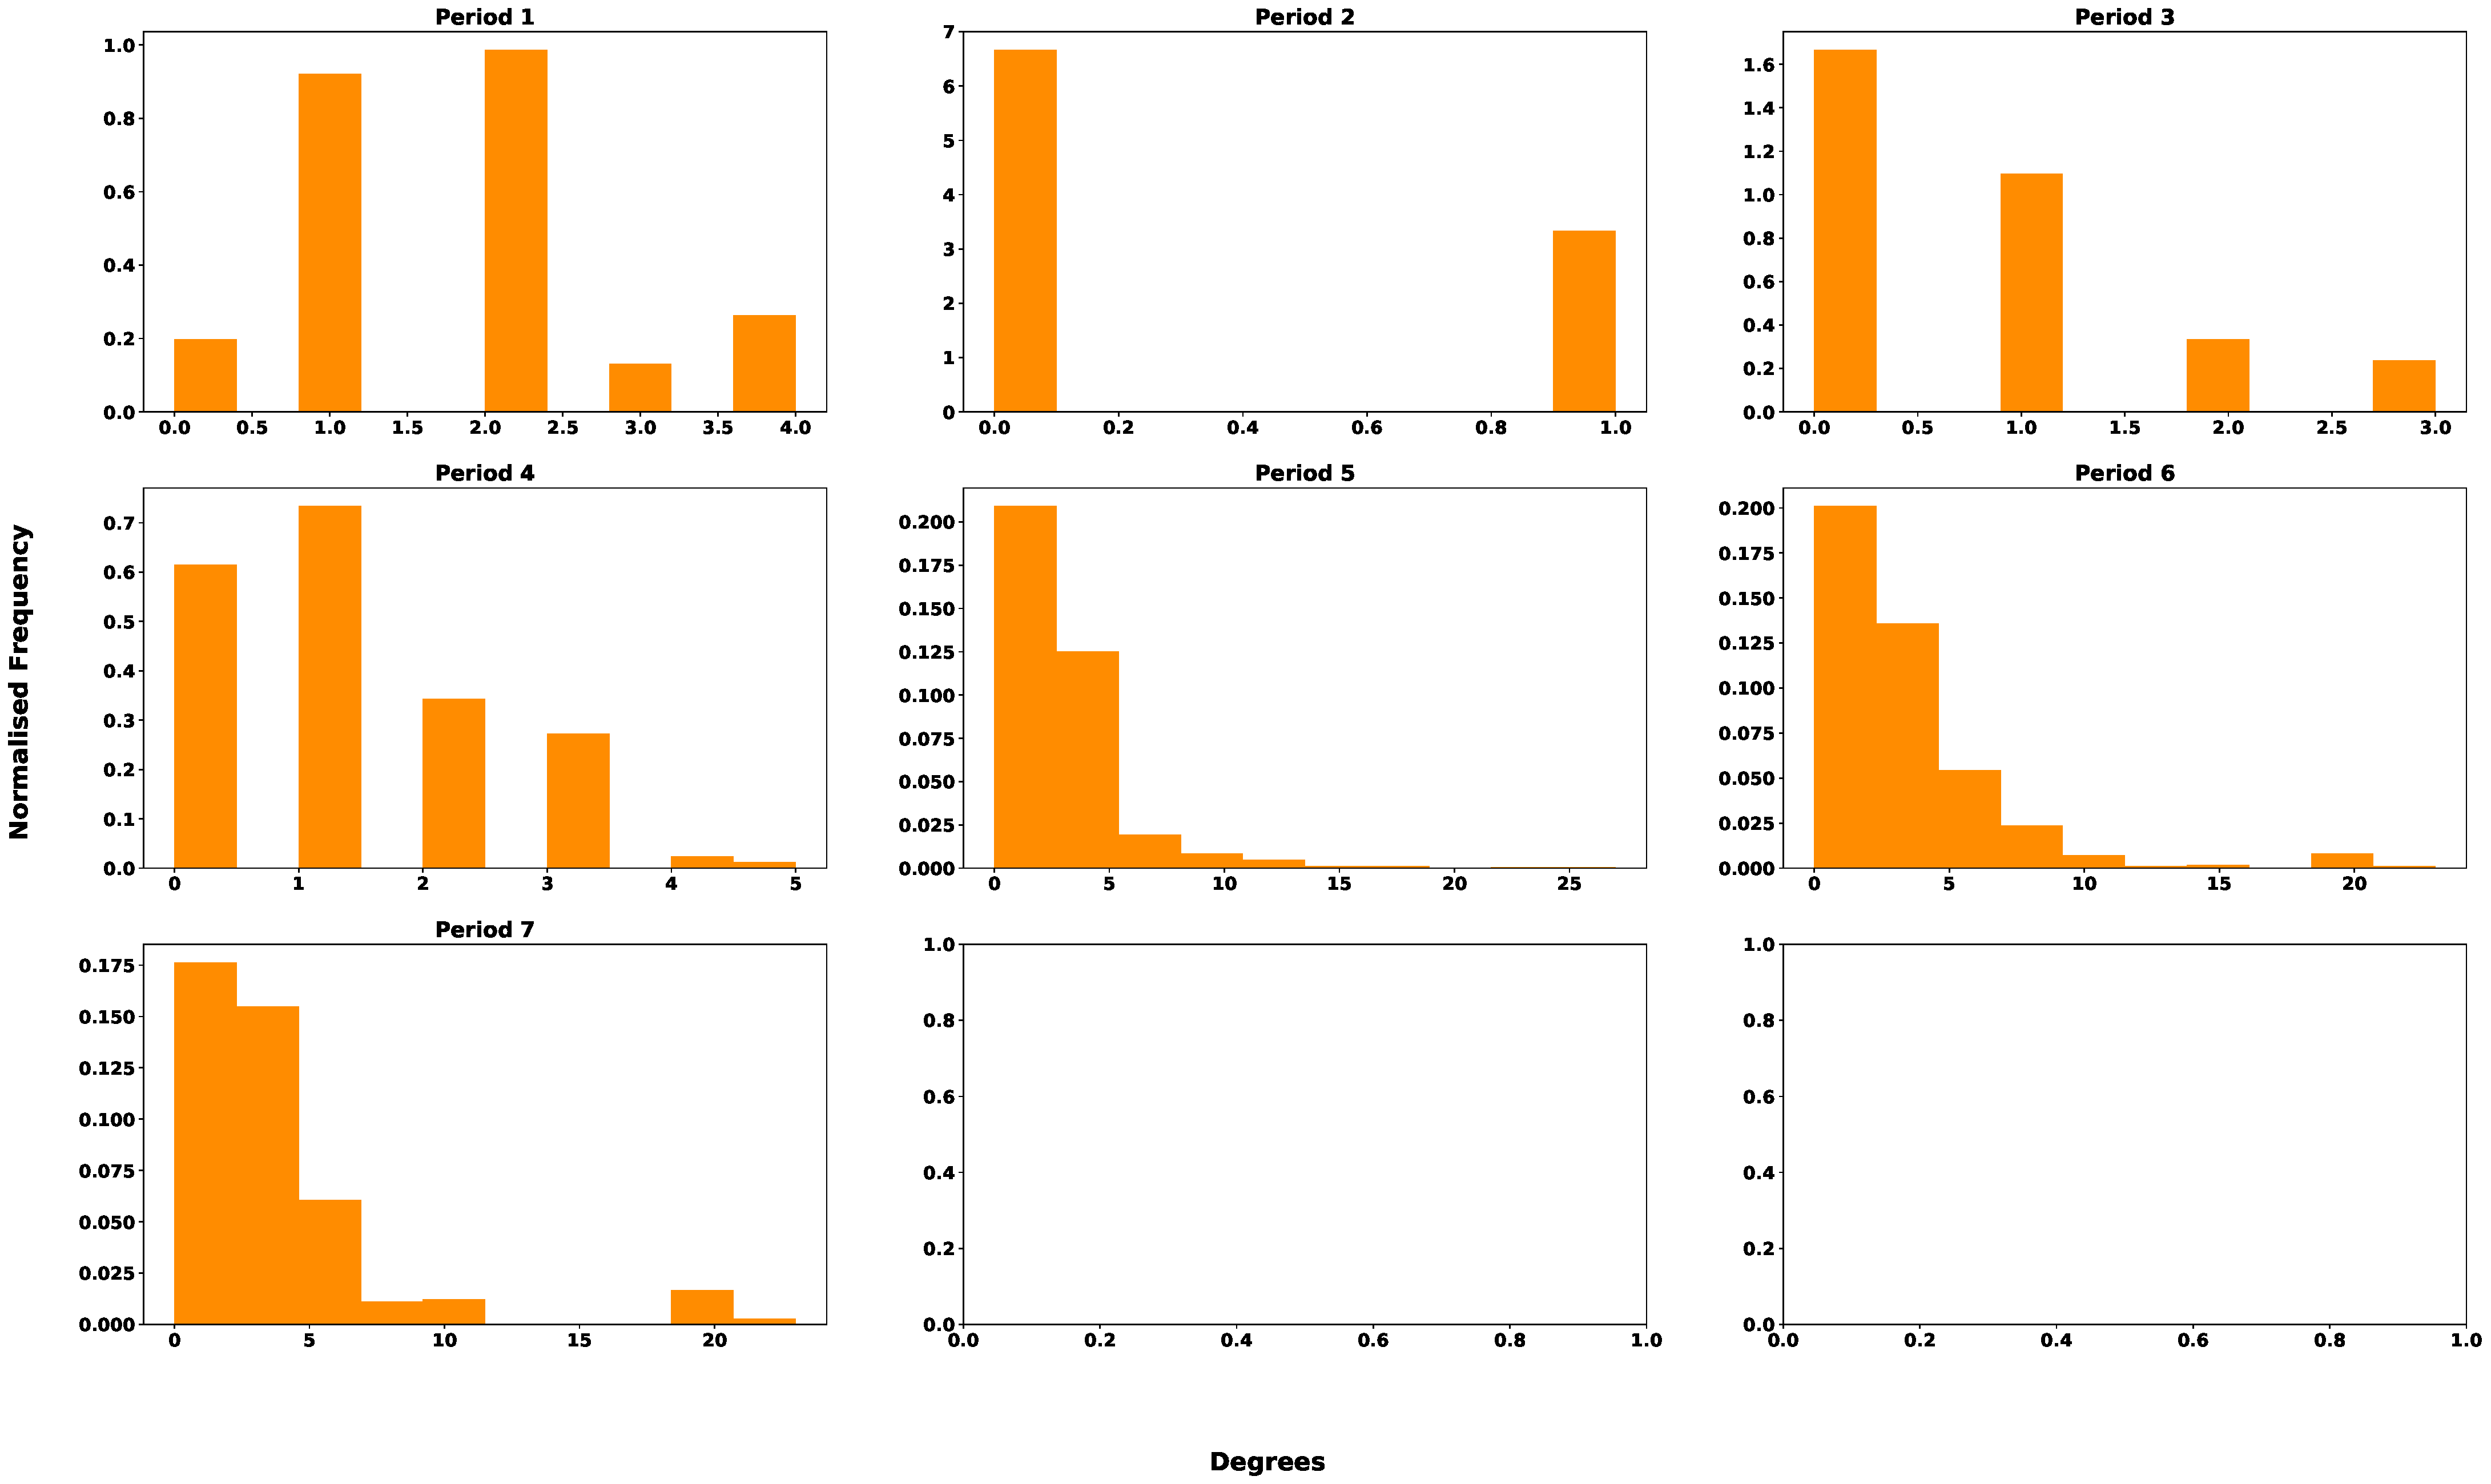
\includegraphics[width=0.8\textwidth]{./assets/images/degrees_histrograms_temporal.pdf}
%     \caption{Degrees distribution over time.}\label{fig:dist_over_time}
% \end{figure}

\subsubsection{Measures of Influence}

Network centrality is used in network theory to study which nodes of a graph are
the most important. There are several centrality measures used to explain different
behaviours of the nodes. Centrality will be used here to explain influence. 
The two centrality which are used are:

\begin{itemize}
    \item Closeness centrality \(C_C\).
    \item Betweenness centrality \(C_B\).
\end{itemize}

Both network measures are explained with an example. The definitions for both
centralities are given by Definition~\ref{def:closeness} and~\ref{def:betweenness}.

\begin{definition}{Closeness.}\label{def:closeness}
    Closenesse centrality of a node \(u\) is the reciprocal of the average
    shortest path distance to \(u\) over all \(n-1\) reachable nodes. It is denoted as,
    
    \[C_C(u)= \frac{n - 1}{\displaystyle \Sigma_{v=1}^{n-1}d(v, u)}\]
    
    where \(d(v, u)\) is the shortest-path distance between \(v\) and \(u\), and \(n\)
    is the number of nodes that can reach \(u\). The mornalised centrality
    is \(C_C\) normalised by the number of nodes in the connected part of the
    graph.
\end{definition}

\begin{definition}{Betweenness.}\label{def:betweenness}
Betweenness centrality of a node \(u\) is the sum of the fraction of all-pairs of
shortest paths that pass through \(u\). It is denoted as,

\[ C_B(u)=\Sigma_{s,t \in V} \frac{\sigma (s,t|u)}{\sigma(s,t)}\]

where \(V\) is the set of nodes, \(\sigma(s,t)\) is the number of shortest \((s,t)\)-paths,
and \(\sigma(s,t|v)\) is the number of those paths passing through some node
\(u\) other than \(s,t\). If \(s=t\), \(\sigma(s,t)=1\), and if \(u \in s,t, \sigma(s,t|u)=0\).
Normalised \(C_B\) is normalized by \(\frac{2}{((n-1)(n-2))}\)
\end{definition}

Closeness is a measure that shows how well a node connects other nodes. Equivalently,
how well an author is connected to other authors and contributes to them collaborating. 
On the other hand betweenness is about how connected a
node is, thus how much influence an author can gain from their environment.

As an example consider a sub graph of \(G_1\) which is illustrated in
Figure~\ref{fig:subgraph_t}. Note that nodes 1, 2 and 3 are connected to three
authors. Thus we expect their betweenness centrality to be the same. However, this
is not true for closeness centrality. Node 3 is the connecting link between at least
4 people. Thus node 3 is the person in the sub graph that influences most authors.
Node 3 also gains influence due ot its rule in the team, but node 2 achieves the
same without connecting people as much as node 3.

\begin{figure}[!hbtp]
    \centering
    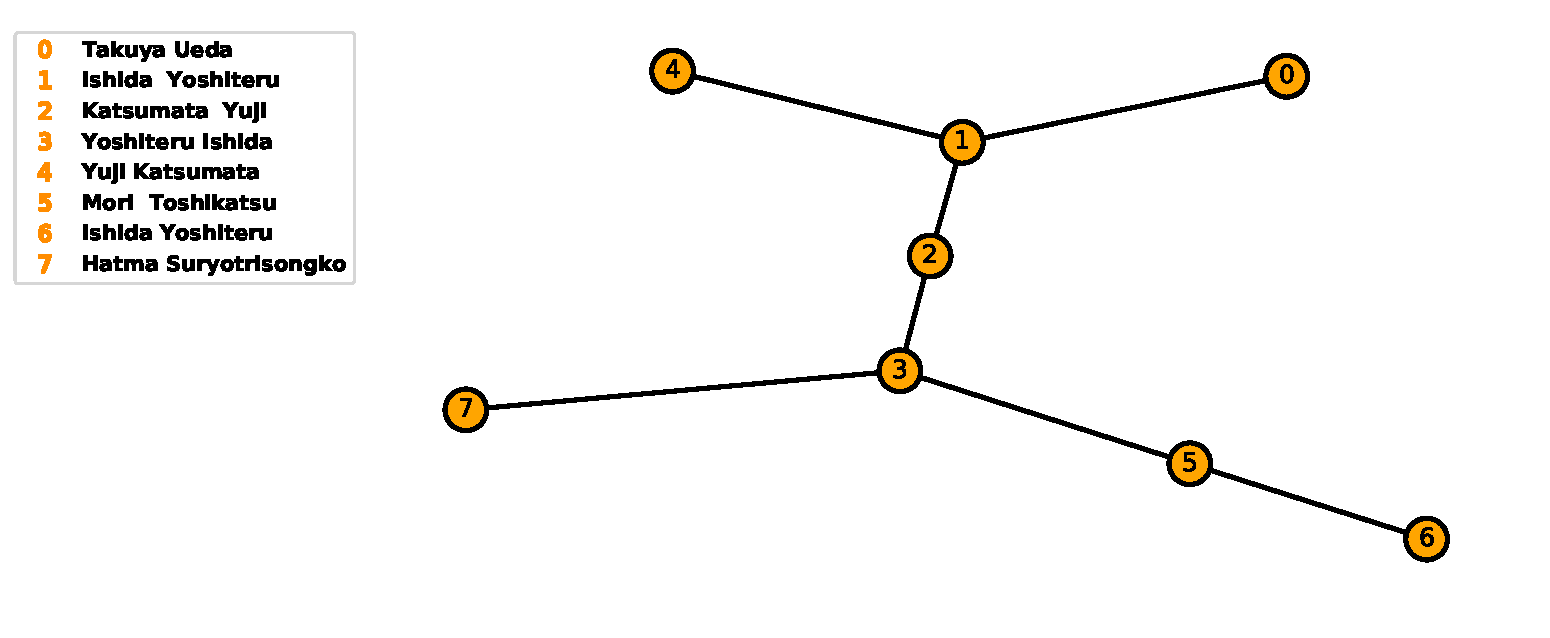
\includegraphics[width=0.8\textwidth]{./assets/images/centrality_example.pdf}
    \caption{A sub graph of \(G_1\).}\label{fig:subgraph_t}
\end{figure}

The centrality for all three networks are calculated using~\cite{networkx}. Table
\ref{table:central_authors_pd} summarises the most important authors of network
\(G_1\) based on the two centralities. The people that influence the field the
most are Matjaz Perc, Yamir Moreno, Luo-Luo Jiang, Arne Traulsen and Martin A.
Nowak. Their work have been discussed in Section~\ref{section:timeline}.
%Examples of their works.
Though Matjaz Perc and Yamir Moreno appear to both influence and gain from
the networks influence, it does not hold for the rest of the three authors.

\begin{table}[!hbtp]
    \begin{center}
    \scalebox{0.8}{
    \begin{tabular}{llr}
\toprule
{} &      Author name &  Betweeness \\
\midrule
1 &      Matjaz Perc &    0.010584 \\
2 &     Yamir Moreno &    0.008786 \\
3 &    Luo-Luo Jiang &    0.004319 \\
4 &    Arne Traulsen &    0.003920 \\
5 &  Martin A. Nowak &    0.003832 \\
\bottomrule
\end{tabular}

    \begin{tabular}{llr}
\toprule
{} &    Author name &  Closeness \\
\midrule
0 &    Matjaz Perc &   0.044428 \\
1 &   Yamir Moreno &   0.043561 \\
2 &   Cheng-Yi Xia &   0.038910 \\
3 &  Sandro Meloni &   0.037959 \\
4 &  Alberto Aleta &   0.037600 \\
\bottomrule
\end{tabular}
}
    \caption{Top 5 ranked authors of \(G_1\) based on different centrality measures.}
    \label{table:central_authors_pd}
    \end{center}
\end{table}

\paragraph{Analysis}
\mbox{ }\\

Influence for a given network is calculated easily. However, we want to assert
the power of the influence of \(G_1\) by comparing the results to those of
\(G_2\) and \(G_3\). Using the distribution of the centralities will we
statistically tests whether a difference does exist between them.

For \(C_C\) all distributions are not normally distributed so we will use the
non parametric test Kruskal Wallis. The test returns a \(p\) value of 0.0 thus 
it can be stated with 95\% confidence of that the distributions are statistically
different. These are plotted as violin plots in Figure~\ref{fig:closeness_dist}.

Note that the centrality values range between 0 and 1. For all three graphs \(C_C\)
have low values. Both \(G_1\) and \(G_2\) appear to have a similar distributions.
Most authors have have a coefficient of zero and a few authors by the tails
appear to have a larger coefficient. This means that for the two topics, the highest
frequency of authors have a very small influence in their field. Though there 
are people with a high influence they are only a few.

The coefficients of \(G_3\) are different from the other topics. Overall it
can be seen that authors' centrality is more spread through the different values.

\begin{figure}[!hbtp]
    \centering
    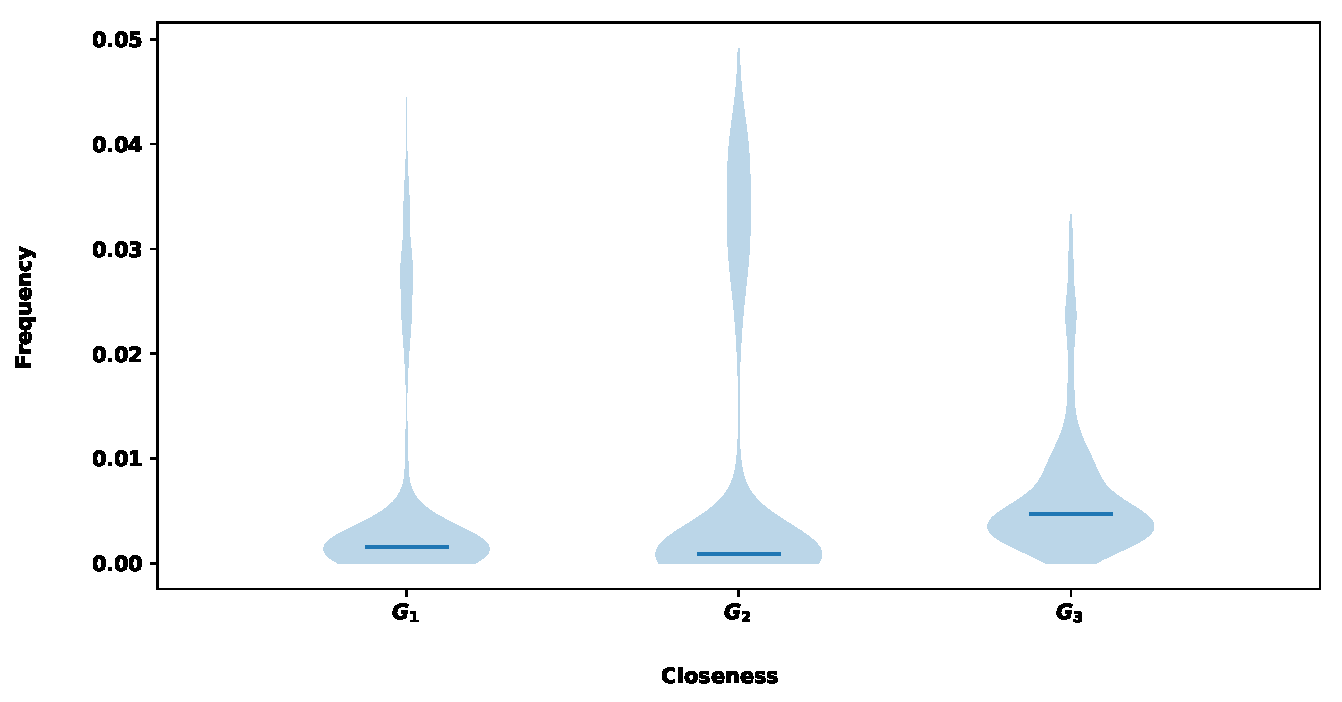
\includegraphics[width=.8\textwidth]{./assets/images/Closeness_histrograms.pdf}
    \caption{Closeness distributions for all three networks.}\label{fig:closeness_dist}
\end{figure}

Figure~\ref{fig:closeness_dist} shows that all coefficients are clustered around the value of zero.

\begin{center}
\begin{figure}[!hbtp]
    \centering
    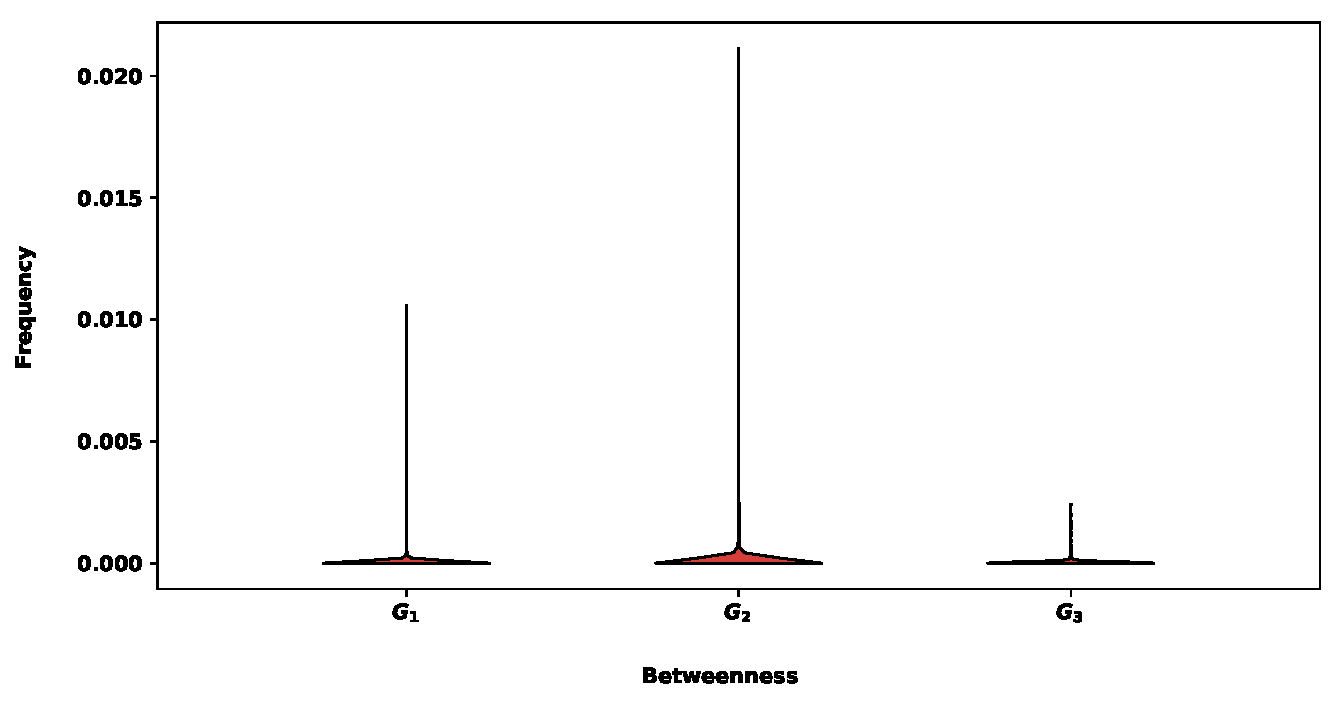
\includegraphics[width=.8\textwidth]{./assets/images/Betweenness_histrograms.pdf}
    \caption{Betweenness distributions for all three networks.}\label{fig:closeness_dist}
\end{figure}
\end{center}

% \paragraph{Temporal comparison}
% \mbox{ }\\

% The two centralities are also studied over time. Table~\ref{table:cc_over_time} higlights
% the authors with the most influnce at each time period. Equivalently, Table~\ref{table:bc_over_time}
% highlights the authors that gained more from the networks' influence at each
% time period.

% For periods 1, 3, 4, 5 and 6 the authors with the highest closeness centrality
% are the authors with the highest betweenness centrality as well. Several of these
% authors have been shown to also have a strong influence to the entire network
% as well.

% For period 7 though March Harper is the person that influences most authors,
% Chen Yi Xia is the person that gains the most. For period 2 we have a similar
% case. Robert Axelrod appears to be the most influenced author but not gaining 
% as much from it.

% Note that the centrality values are decreasing over the time periods. This could
% be an effect due the size of the network which is increasing. In smaller networks
% authors have more motivation to collaborate with the few people on their fields.

% \begin{table}[!hbtp]
%     \begin{center}
%     \scalebox{0.8}{
%     \begin{tabular}{llr}
\toprule
{} &      Author name &  Closeness \\
\midrule
1 &  Svenn Lindskold &   0.108108 \\
2 &       R. Axelrod &   0.200000 \\
3 &  Martin A. Nowak &   0.043478 \\
4 &  Lee A. Dugatkin &   0.029762 \\
5 &      Matjaz Perc &   0.043443 \\
6 &     Yamir Moreno &   0.039311 \\
7 &      Marc Harper &   0.049462 \\
\bottomrule
\end{tabular}
}
%     \caption{Authors with the most influnce at each time period.}
%     \label{table:cc_over_time}
%     \end{center}
% \end{table}

% \begin{table}[!hbtp]
%     \begin{center}
%     \scalebox{0.8}{
%     \begin{tabular}{llr}
\toprule
{} &      Author name &  Betweeness \\
\midrule
0 &  Svenn Lindskold &    0.006006 \\
1 &     A. W. Tucker &    0.000000 \\
2 &  Martin A. Nowak &    0.001279 \\
3 &  Lee A. Dugatkin &    0.000499 \\
4 &      Matjaz Perc &    0.010689 \\
5 &     Yamir Moreno &    0.005468 \\
6 &     Cheng-Yi Xia &    0.001242 \\
\bottomrule
\end{tabular}
}
%     \caption{Authors that gained more from the networks influence at each
%     time period.}
%     \label{table:bc_over_time}
%     \end{center}
% \end{table}

\subsubsection{Conclusion}

In this section we have conducted an investigation of the literature based on a
data analysis. More specifically, this was mainly done using network theory.

Initially, we gave a summary on the data collection. An open source project which was
developed for the purpose of this work was used~\cite{nikoleta_2017}. The project
takes advantage of the API system several academic journals offer today. The
procedure, the sources as well as the keywords used in the process of collection
have been clearly specified making the process reproducible.

Three data sets have been composed for three different topics of game theory.
These are:

\begin{itemize}
    \item The prisoner's dilemma. The main focus of this paper.
    \item Auction games. A sub field of game theory used for comparison reasons.
    \item The price of anarchy. A sub field of game theory used for comparison reasons.
\end{itemize}

We conducted a brief preliminary analysis on these data sets. Mainly to understand
the sizes, provenance and trends of each topic. The main data set was also partitioned
into time periods such that an temporal comparison could be conducted.

The main focus of the analysis has been to explain collaborative behaviour and
influence. Both terms have been defined and we have explained how network measures
of the co authorship network were used to quantify them. The co authorship
network is a network representing all the unique authors of a topic. An edge
exists within two authors if they have written together. Co authorship was
decided to be used as be believe other measures, such as citations, perform less
well.

% The findings of this analysis are presented in two parts. The comparison of the
% collaborative behaviour and influence of the prisoner's dilemma field based on
% other topics and how these measures change for the field over time.

All three networks have been disjointed with a large number of connected components.
The collaborative behaviour was based on the nature of these connected components.
The median connection of an author has been the same for all three networks.
However, the price of anarchy had a smaller number of authors that prefer to write
on their own and based on the clustering coefficient the collaboration of the
field authors appears to be stronger. The collaboration for both the prisoner's
dilemma and auction games it's similar. Note though that the price of anarchy
is a new topic with less authors. It makes more sense for a few people that
work on the topic to be more collaborative which each other.

Similarly influence was studied using two centrality measures. For \(G_1\) and
\(G_2\) we conclude that there are only a few authors that have power of influence
on the network. For research this is not ideal. It could mean that the research
is only driven from the work of specific people. It could also indicate a hostile
environment for new authors. In comparison, \(G_3\) has several authors that have
different influence on their neighbours. A wider spread of influence could indicate
a nice flow of knowledge across the field from different people. This could
help the growth of a field and accelerate findings. The influence that authors
gain from the respective networks was also explored. The results argued that
the gain was very low for all three networks.

% Collaborations and influence of the field have changed over time. As argued
% by~\cite{Etzkowitz1992} over time the amount of research groups was increasing
% for the topic. However, as stated earlier, as the number of researchers increases
% the amount of influence and collaboration decreases. This is because researchers
% can not have full knowledge of their entire network and the more people the network
% has the more people we actually do not know. The results from the temporal
% analysis imply that this is true for the field of the prisoner's dilemma.


\newpage
\bibliographystyle{plain}
\bibliography{bibliography.bib}
\end{document}
